\documentclass[runningheads]{llncs}

\usepackage[T1]{fontenc}
\usepackage{graphicx}
\usepackage{url}
\usepackage{longtable}

\begin{document}

\title{Correlation between economic, health, and institutional context of applicants' country and INZ student visa approval decisions}
\titlerunning{Context and INZ Student Visa Approval Decisions}

\author{Vitalii Kaplan}
\authorrunning{V. Kaplan}
\institute{\email{vitalii.v.kaplan@gmail.com}}

\maketitle

\begin{abstract}
This article examines country-level variation in Immigration New Zealand fee-paying student visa approval rates for the 2022--2025 period. The study combines publicly available INZ decision data with publicly available country-level reference variables from the World Bank, the World Health Organization, and UN M49 regional classifications. The analysis uses descriptive statistics, Pearson correlations, linear regression approximations, alternative regional specifications, residual diagnostics, and a weighted robustness check based on log-transformed application volume.

The results show that approval rates vary systematically across applicant nationalities and are associated with application volume, income classification, regional classification, and broader country-level development indicators. In the modelling table, several health, income, internet-use, mortality, and life-expectancy indicators are strongly correlated with approval rates, although these indicators also overlap substantially with one another. Among the tested regression specifications, the UN M49 regional model has the strongest fit, followed by the World Bank regional model, the WHO regional model, and the no-region model. A weighted UN M49 experiment gives similar overall fit but weakens several individual regional coefficients, supporting the model-fit conclusion while limiting interpretation of particular coefficients.

The findings should be interpreted as country-level descriptive evidence, not as causal evidence about individual visa decisions. The analysis is explicitly based on INZ's published visa instructions, which set out common formal requirements for student visa applicants, including evidence of enrolment, tuition arrangements, sufficient funds, bona fide temporary-entry intent, and relevant health and character requirements. The observed country-level differences are therefore not interpreted as evidence of officer behaviour, discriminatory intent, bias, or unequal treatment in individual application assessment. Rather, they are treated as aggregate descriptive outcomes that may reflect country-level differences in documentary, financial, institutional, and verification conditions under the same formal decision framework. The principal limitation is that the data are aggregated by country and do not include applicant-level records, programme choice, education provider information, documentation quality, or detailed processing factors. The study identifies a reproducible empirical structure and points to further research on other receiving countries, additional country-level variables, and formal inter-country education or migration relationships.

\keywords{student visas \and Immigration New Zealand \and country-level analysis \and approval rates \and regional classification}
\end{abstract}

\section{Introduction}

International student mobility is now a large but unevenly distributed part of higher education. UNESCO reports that 6.9 million higher-education students study outside their home country, more than three times the number in 2000 \cite{UNESCO2025}. New Zealand is a small destination in this global system, but not a marginal case for its own economy. In 2024 it had 50,300 international tertiary learners, approximately 0.7 percent of the global internationally mobile higher-education population if compared with UNESCO's 6.9 million figure \cite{TEC2024Snapshot,UNESCO2025}. Across all education sectors, New Zealand recorded 83,425 international student enrolments in 2024 \cite{ENZ2025Enrolments}. The Government's international education plan identifies the sector as a major export activity and aims to increase its value from NZ\$3.6 billion in 2024 to NZ\$7.2 billion by 2034 \cite{MoEInternationalEducation}.

New Zealand is therefore a useful empirical setting for studying student visa decisions. It is geographically isolated, relatively small, and economically interested in international education, so student entry is both commercially important and administratively filtered. A fee-paying student visa application is not a casual expression of interest. INZ's published instructions require evidence and documents concerning enrolment, tuition arrangements, sufficient funds, bona fide temporary-entry intent, and relevant health and character matters \cite{INZEvidence}. Appendix~\ref{app:student-visa-preparation} summarises the preparation steps that make these applications document-intensive. The process is costly and document-intensive, so the observed applications are unlikely to be dominated by low-effort or ``noise'' submissions. Applicants usually need to have already assembled institutional, financial, and personal evidence before a decision appears in the published visa statistics.

The empirical problem is that approval rates differ by applicant nationality, but the reasons for these differences are not visible in the public INZ decision tables. The published rules used in this article state common formal requirements; they do not state separate approval rules by nationality. For this reason, observed country-level differences should not be treated as direct evidence of unequal treatment in individual assessment. They are better framed as an aggregate empirical pattern that may reflect differences in application volume, documentation conditions, financial evidence, institutional context, verification conditions, or other country-level circumstances under a common formal decision framework.

The research question is narrow: are country-level INZ fee-paying student visa approval rates for 2022--2025 associated with application volume, national development and health indicators, income classification, and alternative regional classifications? The article answers this question by joining public INZ decision data to public World Bank, WHO, and UN M49 reference data and by comparing descriptive statistics, correlations, and regression approximations across alternative regional specifications.

Previous quantitative research on international student migration has used visa refusal or visa-policy data together with student mobility or enrolment outcomes, particularly in the United States and Canada. Chen examines U.S. F-1 visa restrictiveness and international student enrolment, while Gonnot studies Canadian student visa policy and community-college enrolment \cite{Chen2023,Gonnot2025}. Other work models international student mobility using origin- and destination-country characteristics, including World Bank development indicators. However, peer-reviewed work directly modelling New Zealand student visa approval rates appears limited, and studies combining country-level student visa decision data with both World Bank development indicators and WHO health indicators are also uncommon. This article addresses that gap with a reproducible country-level descriptive design.

\section{Literature Review}

\begin{quote}
\emph{Some are born to Sweet Delight,\\
Some are born to Endless Night} \cite{Blake1863}.
\end{quote}

International education is often presented as an open global market in which students choose programmes and institutions compete for talent. This framing hides a basic constraint: students cannot simply choose to study abroad unless a state permits them to enter and remain. Cross-border education is therefore not only an academic or economic process; it is also a migration process governed by visa systems. Sassen notes that international law does not provide a general right to enter foreign territory \cite{Sassen1996}. Shachar similarly emphasises that the practical value of citizenship is closely tied to mobility rights attached to passports \cite{Shachar2014}. Visa systems therefore sit at the boundary between education markets and state control over entry.

This matters because mobility is unevenly distributed. Neumayer argues that states use visa restrictions to manage a trade-off between facilitating entry for some passport holders and deterring others for reasons of security, immigration control, economic interest, and political interest \cite{Neumayer2006}. Mau develops a related account of the global mobility divide, in which visa policies produce unequal access to cross-border movement \cite{Mau2015}. In this literature, visa policy is not a neutral background condition. It is one of the central mechanisms through which access to international mobility is facilitated for some groups and constrained for others.

International student mobility is part of this wider mobility system. Oduwaye reviews the challenges faced by international students and shows that financial stability and other adaptation conditions remain central issues across host countries \cite{Oduwaye2023}. Gulel describes visa inequities in academic mobility and treats visa access as a form of privilege rather than a purely administrative step \cite{Gulel2025}. These studies support the premise that international education cannot be analysed only through enrolment demand or university admission. For many applicants, admission to a programme is only one step in a longer chain of documentary, financial, institutional, and immigration requirements.

The New Zealand case is relevant because international education is a policy and economic sector, while student entry remains governed by formal visa requirements. Craymer reports New Zealand's policy aim to expand the international education market substantially by 2034 \cite{Craymer2025}. At the same time, Spoonley discusses contemporary immigration policy challenges in New Zealand, and Bonnett reports concerns about Immigration New Zealand's processing systems and risk capacity \cite{Spoonley2025,Bonnett2024}. INZ's published student visa instructions require applicants to provide evidence and documents, including enrolment, tuition arrangements, sufficient funds, bona fide temporary-entry intent, and relevant health and character information \cite{INZEvidence}. Appendix~\ref{app:student-visa-preparation} summarises the preparation steps that make these applications document-intensive. These formal requirements make the student visa decision process a suitable empirical setting for studying how country-level conditions may appear in aggregate approval-rate patterns.

Existing quantitative migration research provides methodological precedents for joining migration-related outcomes with country-level indicators. Weber examines the relationship between development and international student migration, showing that student mobility can be studied as part of broader development and migration transitions \cite{Weber2023}. Bertoli uses international migration data joined with macroeconomic sources and highlights the importance of modelling migration in relation to multiple country-level contexts \cite{Bertoli2013}. Abbott applies ordinary least squares regression in a gravity-model framework for international student migration and uses country-level variables to explain student flows \cite{Abbott2016}. These studies differ from the present analysis in outcome and design, but they support the use of country-level explanatory variables and regression-based approximation for migration-related questions.

Prior research also shows that visa policy and approval patterns can shape international student mobility. Chen studies U.S. F-1 visa restrictiveness and international student enrolment, while Gonnot examines Canadian student visa policy and international student migration \cite{Chen2023,Gonnot2025}. Gonnot is especially relevant because it links lower study-visa approval rates for applicants from developing countries to information and documentation problems that may fail to resolve immigration officers' concerns \cite{Gonnot2025}. This supports the present article's cautious interpretation: lower approval rates need not be read as evidence of unequal person-to-person treatment; they may reflect differences in the evidence available to satisfy formal visa requirements.

Country-level and regional explanations are also supported by the broader student-mobility literature. Perkins and Neumayer, Abbott, Bessey, and Lanati and Thiele use country-level data to analyse determinants of international student flows, including geographic factors, networks, institutional quality, political freedom, GDP per capita, fees, and foreign aid projects \cite{PerkinsNeumayer2014,Abbott2016,Bessey2012,LanatiThiele2020}. This literature justifies treating student mobility and visa outcomes as phenomena that can be associated with country-level conditions, while also showing that such models cannot identify all applicant-level mechanisms.

Some related research examines unequal outcomes in labour-market or social settings. Hersch studies the relationship between skin colour and immigrant labour-market outcomes in the United States, and Oreopoulos uses a field experiment to examine discrimination against applicants with foreign experience or non-English names \cite{Hersch2008,Oreopoulos2011}. These studies are not direct models of INZ student visa decisions and are not used here to infer bias in visa assessment. Their relevance is narrower: they show that observed outcomes involving migrants can vary by origin-linked characteristics, and that empirical work must be careful to distinguish documented unequal treatment from aggregate differences that may arise through other mechanisms.

The present article contributes to this literature by analysing publicly available INZ fee-paying student visa decision data at country level and joining it with publicly available World Bank, WHO, and UN M49 reference data. Previous studies have used visa restrictiveness, student mobility, enrolment, or country-level development variables, but peer-reviewed work directly modelling country-level student visa approval rates with both development and health indicators appears limited. The analysis therefore addresses a specific empirical gap: whether country-level approval-rate variation in New Zealand student visa decisions is associated with application volume, national development indicators, income classification, and alternative regional classifications.

\section{Data}

The primary source data are publicly available Immigration New Zealand offshore or overseas student visa decision tables for 2022, 2023, 2024, and 2025 \cite{INZ2022,INZ2023,INZ2024,INZ2025}. The project repository is available on GitHub \cite{KaplanINZRepo}; all file paths in this article are repository-relative paths. The source files are stored in \texttt{data/original/} and are not edited manually. They report fee-paying student visa decisions by applicant nationality or country. The yearly files use slightly different column names, but the common information is the country or nationality, number approved, number declined, total or volume of applications, approval rate, and decline rate.

The unit of observation in the prepared INZ table is a country or applicant nationality aggregated across the four-year period. The unified prepared file, \texttt{data/prepared/inz\_student\_visa\_decisions\_2022-2025.csv}, contains 179 countries or applicant nationalities. For each row it reports total approvals, total declines, total applications, approval rate, and \texttt{Applications\_log10}, the base-10 logarithm of total applications. Approval rate is calculated as approved applications divided by total applications. This table is used for descriptive results on application volume and overall approval rates.

The modelling dataset joins the prepared INZ table to publicly available country-level reference data from the World Bank, the World Health Organization, and UN M49 \cite{WorldBankWDI,WorldBankCLG,WHOData,WHOGHO,UNM49}. The World Bank reference table contributes FY2026 region, income group, lending category, GDP per capita, GNI per capita using the Atlas method, life expectancy, internet-use percentage, and urban-population percentage. The WHO reference table contributes WHO region, under-five mortality, maternal mortality, DTP3 immunization coverage, and physician density. The UN M49 reference table contributes an alternative regional classification.

Country names are harmonised across the INZ, World Bank, WHO, and UN M49 files before modelling. The combined modelling file is \texttt{data/prepared/inz\_2022-2025\_wb\_who\_m49\_combined.csv}. It contains 110 countries after country matching, removal of rows with missing numerical values needed for the models, and exclusion of countries with fewer than 10 total applications across 2022--2025. Countries present in the prepared INZ table but absent from the regression table are reported separately in \texttt{data/support/Countries\_excluded\_from\_regression.csv}.

The repository \cite{KaplanINZRepo} distinguishes source, prepared, combined, and result files. Source files in \texttt{data/original/} preserve the downloaded INZ and reference tables. Prepared files in \texttt{data/prepared/} contain harmonised and joined datasets used for analysis. Result files in \texttt{data/results/} contain model coefficients, scores, predictions, prediction-rate tables, and correlation outputs. Support files in \texttt{data/support/} contain derived diagnostic summaries and auxiliary tables used to interpret the results.

\section{Methods}

\subsection{Computational Workflow}

The analysis was implemented as a set of KNIME workflows and exported Python workbooks. The repository contains three main KNIME workflows: \texttt{INZ\_visa\_decisions\_unification}, \texttt{INZ\_visa\_decisions\_combined}, and \texttt{INZ\_visa\_decisions\_model}. The workflow directories preserve the original KNIME node structure, while the corresponding \texttt{.py} and \texttt{.ipynb} files provide a text-based computational record. The Python files were generated from the KNIME workflows by the open-source \texttt{knime2py} utility available through \texttt{k2pweb.org}. They are treated here as exported translations of the KNIME workflows rather than as independent alternative analyses.

The unification workflow reads the yearly INZ decision files for 2022, 2023, 2024, and 2025, harmonises differences in column names, keeps the common decision fields, concatenates the yearly tables, and aggregates them by country or applicant nationality. It calculates total approvals, total declines, total applications, approval rate, and \texttt{Applications\_log10}. The combined-data workflow joins this prepared INZ table to the World Bank, WHO, and UN M49 reference tables after country-name harmonisation. It removes unusable columns, records missing string categories where needed, removes rows with missing numerical values required for modelling, and exports the combined modelling table and correlation output.

The modelling workflow reads \texttt{data/prepared/inz\_2022-2025\_wb\_who\_m49\_combined.csv}. Numerical explanatory variables are min--max normalised before fitting. Categorical predictors, including income, lending-category, and regional variables, are represented as indicator variables with one category omitted as the reference level. The dependent variable is country-level approval rate. The model outputs are written to \texttt{data/results/} as coefficient tables, fitted-value tables, prediction-rate tables, and score tables. Additional support scripts produce robustness and residual summaries used in the sensitivity checks.

\subsection{Descriptive Statistics and Regression}

The first stage is descriptive. The unified INZ table is used to report the number of countries or applicant nationalities, total applications, approval rates, and the distribution of application volume. Application volume is represented both as total applications and as \texttt{Applications\_log10}, because application counts are highly uneven across countries.

Associations between approval rate and individual country-level variables are examined with Pearson correlation coefficients. These correlations are reported with the correlation coefficient, p-value, and degrees of freedom where relevant. They are used for the relationship between approval rate and application volume, and for relationships between approval rate and country-level indicators such as mortality, life expectancy, internet use, physician density, GNI per capita, and GDP per capita.

The main modelling step uses ordinary least squares linear regression to approximate country-level approval rate as a function of selected WHO and World Bank indicators, income and lending categories, and, in three specifications, regional classification variables. The models are explanatory approximations. They are not operational prediction systems and are not causal designs. Their purpose is to measure how much of the observed country-level variation can be fitted by the current set of country-level variables.

\subsection{Regional Specifications}

The country-level numerical variables and the regional variables have different methodological status. Health, income, internet-use, mortality, and life-expectancy measures are treated as country-level reference indicators. For a given source and year, these variables have a defined value for a country. Regional classification is different. A region is an external grouping imposed on countries, and the same country can be assigned to different regional systems depending on the classification scheme. For this reason, regional division is treated as a modelling choice rather than as an inherent property of the country.

The analysis estimates four related specifications. Three models use alternative external regional classifications: UN M49 regions, World Bank FY2026 regions, and WHO regions. A fourth model excludes regional variables. The same dependent variable and the same non-regional country-level predictors are used across the specifications, so the comparison focuses on whether the choice of regional grouping changes model fit. This design separates two questions: whether country-level reference indicators are associated with approval rates, and whether an external regional classification adds explanatory structure beyond those indicators.

\subsection{Model Evaluation and Residuals}

The regression models are evaluated with standard linear model fit statistics. The main comparison across model specifications uses R-squared, mean absolute error, mean squared error, and root mean squared error. These statistics are used to compare the UN M49, World Bank regional, WHO regional, and no-region specifications. They measure fit within the current country-level modelling table and should not be read as validation of a causal mechanism.

Individual regression terms are assessed with coefficient estimates and p-values. The p-values are used to identify variables and regional indicators that cross the conventional $p < 0.05$ threshold within each specification. Because the models include correlated country-level indicators and categorical regional variables, statistical significance is interpreted as conditional association within the fitted model rather than as evidence of an independent causal effect.

Prediction diagnostics are based on residuals and relative fitted error. Residual summaries include the mean residual, residual standard deviation, mean absolute residual, and maximum absolute residual. Residuals are also inspected against fitted values to check whether unexplained error is concentrated in particular fitted-value ranges. Relative residuals are examined with \texttt{Prediction\_rate}, defined as the ratio of observed approval rate to fitted approval rate. Countries with observed approval rates below 80 percent or above 120 percent of the fitted value are treated as large proportional deviations for descriptive comparison. These cases are not treated automatically as technical outliers; they identify countries where the current variables fit observed approval rates poorly.

\subsection{Robustness and Interpretation}

Robustness checks compare the same quantities across alternative regional classifications and a weighted UN M49 specification. The weighted model uses \texttt{Applications\_log10} as the observation weight, giving more influence to countries with larger log-transformed application volumes. It is evaluated with weighted R-squared, weighted mean absolute error, weighted mean squared error, and weighted root mean squared error, and also with unweighted fit statistics for comparison with the main UN M49 model.

The interpretation of these statistics rests on INZ's published student visa instructions, which define common formal requirements for applicants. The models therefore do not use country-level differences to infer unequal treatment, bias, or discriminatory decision-making. They use those differences to study variation in the conditions under which applicants from different countries prepare, document, finance, and verify applications within the same formal decision framework. The analysis is also limited by the aggregation of applications to country level and by overlap among country-level predictors. The correlation output is therefore used not only as descriptive evidence but also as a warning that individual regression coefficients should not be overinterpreted as independent effects.

\section{Results}

\subsection{Descriptive Results}

The unified INZ decision table contains 179 countries or applicant nationalities and 148,746 total fee-paying student visa applications across 2022--2025. Across these records, the overall approval rate is approximately 81.3 percent.

Application volume is unevenly distributed across countries. The largest application counts are from China, India, Japan, Nepal, the United States of America, Sri Lanka, Germany, Thailand, the Philippines, and South Korea. These high-volume countries do not all have the same approval rate. For example, China, Japan, the United States of America, Germany, and South Korea have approval rates above 96 percent, while India and Nepal have lower approval rates in the current prepared table.

The relationship between application volume and approval rate is positive but not strong. In the unified country-level table, the Pearson correlation between log10 total applications and approval rate is about 0.27, with $p = 0.000254$ and 177 degrees of freedom. This supports a limited descriptive statement: countries with more applications tend to have higher approval rates, but application volume alone does not explain most of the variation in approval rates. Figure~\ref{fig:applications-log10-approval-rate} shows this relationship graphically.

\begin{figure}
\centering
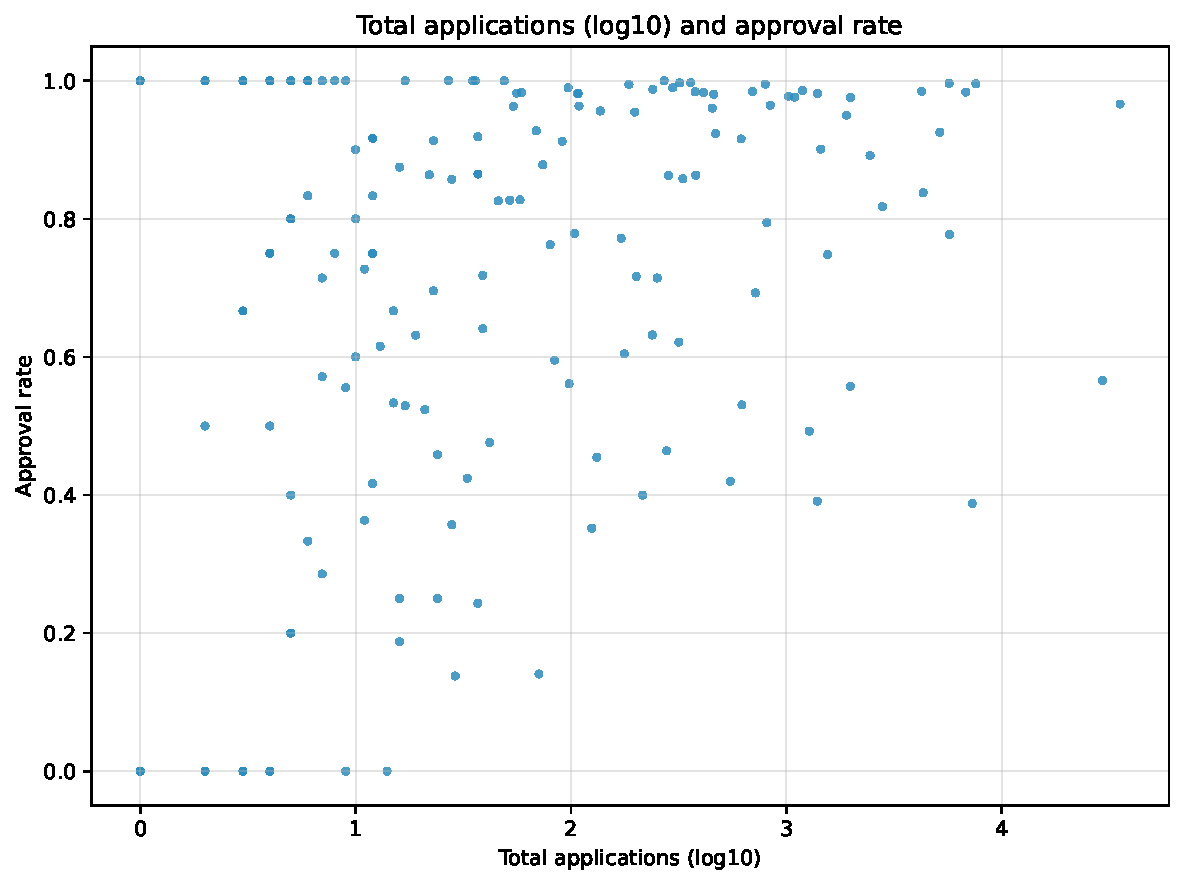
\includegraphics[width=\textwidth]{imgs/applicationslog10_to_approval_rate.pdf}
\caption{Total applications, log10 transformed, and student visa approval rate by country or applicant nationality. The PDF figure is generated from \texttt{data/results/applicationslog10\_to\_approval\_rate.svg}.}
\label{fig:applications-log10-approval-rate}
\end{figure}

\subsection{Correlation With Country-Level Indicators}

After joining the INZ data with WHO, World Bank, and UN M49 reference data, the combined modelling table contains 110 countries. This reduction reflects the availability of matched country-level reference variables, the removal of rows with missing numerical values, and the exclusion of countries with fewer than 10 total applications across the four-year period. The countries excluded before regression modelling are listed in Appendix Table~\ref{tab:appendix-excluded-countries}.

Several country-level indicators are strongly correlated with approval rate. The direction of the correlations is consistent with a broad development and administrative-capacity pattern. Approval rates are lower where mortality indicators are higher, and higher where life expectancy, internet use, physician density, and income indicators are higher. Table~\ref{tab:approval-country-correlations} reports the strongest bivariate correlations used in this interpretation.

\begin{table}
\caption{Correlations between approval rate and selected country-level indicators}
\label{tab:approval-country-correlations}
\centering
\renewcommand{\arraystretch}{1.25}
\setlength{\tabcolsep}{8pt}
\begin{tabular}{lrr}
\hline
Indicator & $r$ & $p$ \\
\hline
WHO under-five mortality per 1,000 live births & -0.746 & $1.24e{-30}$ \\
WHO maternal mortality per 100,000 live births & -0.681 & $7.97e{-24}$ \\
Life expectancy at birth & 0.715 & $4.19e{-27}$ \\
Internet users as percentage of population & 0.633 & $7.62e{-20}$ \\
Physician density per 10,000 population & 0.552 & $1.56e{-14}$ \\
GNI per capita, Atlas method & 0.520 & $8.18e{-13}$ \\
GDP per capita, current USD & 0.501 & $7.42e{-12}$ \\
\hline
\end{tabular}
\end{table}

The same correlation output also shows that several explanatory variables are strongly correlated with each other. For example, WHO under-five mortality is strongly negatively correlated with life expectancy ($r = -0.888$) and internet-user percentage ($r = -0.770$), and strongly positively correlated with WHO maternal mortality ($r = 0.881$). This means that the numerical country-level indicators partly measure overlapping dimensions of national development, health conditions, and institutional capacity.

These correlations indicate that approval rates are associated with broad country-level development, health, and income measures. They should not be read as causal effects. The data are aggregated by country, and the variables describe country-level conditions rather than individual applicants.

This interpretation is limited to formal and administrative conditions surrounding applications. The analysis is explicitly based on INZ's published visa instructions, which set out common formal requirements for student visa applicants, including evidence of enrolment, tuition arrangements, sufficient funds, bona fide temporary-entry intent, and relevant health and character requirements. The observed country-level differences are therefore not interpreted as evidence of officer behaviour, discriminatory intent, bias, or unequal treatment in individual application assessment. Rather, they are treated as aggregate descriptive outcomes that may reflect country-level differences in documentary, financial, institutional, and verification conditions under the same formal decision framework.

\subsection{Regression Approximation}

Four linear regression specifications were estimated. Three specifications use different regional classifications: UN M49, World Bank regions, and WHO regions. A fourth specification excludes regional classification variables. In each case, approval rate is the dependent variable, and the model uses selected WHO and World Bank country-level variables, with or without regional classification variables, as explanatory inputs.

\begin{table}
\caption{Regional classification specifications used in the regression models}
\label{tab:regional-classification-counts}
\centering
\renewcommand{\arraystretch}{1.2}
\begin{tabular}{lr}
\hline
Specification & Number of regions in modelling table \\
\hline
UN M49 regional classification & 21 \\
World Bank FY2026 regional classification & 7 \\
WHO regional classification & 6 \\
\hline
\end{tabular}
\end{table}

The UN M49 specification has the strongest fit among the current models, while the no-region specification has the weakest fit. Table~\ref{tab:model-fit-comparison} reports the fit statistics for all four specifications.

\begin{table}
\caption{Model fit by regional specification}
\label{tab:model-fit-comparison}
\centering
\renewcommand{\arraystretch}{1.2}
\setlength{\tabcolsep}{8pt}
\begin{tabular}{lrrr}
\hline
Specification & R-squared & MAE & RMSE \\
\hline
UN M49 regional model & 0.867 & 0.069 & 0.090 \\
World Bank regional model & 0.812 & 0.082 & 0.107 \\
WHO regional model & 0.786 & 0.087 & 0.114 \\
No-region model & 0.706 & 0.100 & 0.134 \\
\hline
\end{tabular}
\end{table}

These scores suggest that the current country-level variables explain a substantial share of the variation in country-level approval rates, and that regional classification adds explanatory structure to the model. The no-region model still fits a large part of the variation, but all three regional specifications improve fit. The better fit of the UN M49 model may reflect the more detailed regional division used in that specification. This interpretation is supported by the robustness and sensitivity checks described below, but it should remain limited to model fit rather than causal explanation.

The coefficient tables show that model fit is not produced by regional variables alone. Other variables from the combined dataset also contribute to the fitted approval rates. The signs and magnitudes of these coefficients should be interpreted carefully because the model includes correlated country-level indicators and categorical variables. The coefficients show conditional associations within the fitted model, not independent causal effects.

In the UN M49 experiment, only a small set of non-region variables and regional indicators have p-values below 0.05. Table~\ref{tab:un-m49-significant-terms} lists these terms. In this specification, life expectancy remains statistically visible after regional controls are included, while most other numerical country-level indicators do not.

\begin{table}
\caption{Terms below $p < 0.05$ in the UN M49 specification}
\label{tab:un-m49-significant-terms}
\centering
\renewcommand{\arraystretch}{1.2}
\setlength{\tabcolsep}{7pt}
\begin{tabular}{llrr}
\hline
Term & Type & Coefficient & $p$ \\
\hline
Urban population percentage & Variable & -0.279 & 0.0053 \\
Life expectancy at birth & Variable & 0.499 & 0.0128 \\
World Bank lending category: missing & Category & 0.242 & 0.0156 \\
Northern Africa & Region & -0.254 & 0.0109 \\
Middle Africa & Region & -0.275 & 0.0219 \\
Southern Asia & Region & -0.210 & 0.0336 \\
\hline
\end{tabular}
\end{table}

The missing category for World Bank lending category needs a specific interpretation. In the modelling table, all countries in this category are high-income countries. They include countries such as Japan, Singapore, South Korea, Canada, the United States of America, Germany, France, Great Britain, Switzerland, Norway, Sweden, Austria, Belgium, Denmark, Ireland, Italy, Spain, Kuwait, Oman, Saudi Arabia, and the United Arab Emirates. The category therefore should not be read as ordinary data loss. In this dataset, it mainly identifies high-income economies without an assigned World Bank lending category. Its positive coefficient is consistent with the generally high approval rates observed for this group, but it should be interpreted as a proxy for this country group rather than as an effect of missing information.

The negative regional coefficients in Table~\ref{tab:un-m49-significant-terms} also require a categorical interpretation. Regional variables are entered as indicator variables, so each regional coefficient is estimated relative to the omitted reference region, not relative to zero approval or to the global average. A negative coefficient therefore means that, conditional on the other variables in the model, the fitted approval rate for that region is lower than the fitted approval rate for the reference region. It does not mean that the region has a negative approval rate, and it should not be read as an absolute ranking of regions.

The World Bank regional experiment combines income-group effects, urban population percentage, lending-category information, and broad World Bank regional effects. Table~\ref{tab:world-bank-significant-terms} lists the terms below $p < 0.05$ in this specification.

\begin{table}
\caption{Terms below $p < 0.05$ in the World Bank regional specification}
\label{tab:world-bank-significant-terms}
\centering
\renewcommand{\arraystretch}{1.2}
\setlength{\tabcolsep}{7pt}
\begin{tabular}{llrr}
\hline
Term & Type & Coefficient & $p$ \\
\hline
World Bank low-income status & Category & -0.407 & $5.48e{-05}$ \\
World Bank lower-middle-income status & Category & -0.136 & 0.0461 \\
World Bank lending category: missing & Category & 0.224 & 0.0171 \\
Urban population percentage & Variable & -0.255 & 0.0061 \\
\begin{tabular}[c]{@{}l@{}}Middle East, North Africa,\\ Afghanistan and Pakistan\end{tabular} & Region & -0.270 & $8.19e{-08}$ \\
Europe and Central Asia & Region & -0.185 & 0.000369 \\
South Asia & Region & -0.232 & 0.000555 \\
Sub-Saharan Africa & Region & -0.156 & 0.0042 \\
\hline
\end{tabular}
\end{table}

The WHO regional experiment has fewer significant regional terms than the World Bank regional model and a weaker overall fit. Table~\ref{tab:who-significant-terms} lists the terms below $p < 0.05$ in this specification. The Region of the Americas is close to the 0.05 threshold but does not cross it ($p = 0.0691$).

\begin{table}
\caption{Terms below $p < 0.05$ in the WHO regional specification}
\label{tab:who-significant-terms}
\centering
\renewcommand{\arraystretch}{1.2}
\setlength{\tabcolsep}{7pt}
\begin{tabular}{llrr}
\hline
Term & Type & Coefficient & $p$ \\
\hline
World Bank low-income status & Category & -0.442 & $4.23e{-05}$ \\
World Bank lower-middle-income status & Category & -0.178 & 0.0127 \\
World Bank lending category: missing & Category & 0.231 & 0.0198 \\
Urban population percentage & Variable & -0.237 & 0.0132 \\
Western Pacific Region & Region & 0.198 & 0.000975 \\
\hline
\end{tabular}
\end{table}

In the no-region experiment, the model has no regional indicators, so the fit depends only on non-region country-level variables. Table~\ref{tab:no-region-significant-terms} lists the terms below $p < 0.05$ in this specification. These variables carry substantial explanatory information, even though the no-region model fits worse than all three regional specifications.

\begin{table}
\caption{Terms below $p < 0.05$ in the no-region specification}
\label{tab:no-region-significant-terms}
\centering
\renewcommand{\arraystretch}{1.2}
\setlength{\tabcolsep}{7pt}
\begin{tabular}{llrr}
\hline
Term & Type & Coefficient & $p$ \\
\hline
World Bank low-income status & Category & -0.609 & $2.50e{-07}$ \\
World Bank lower-middle-income status & Category & -0.224 & 0.00465 \\
WHO DTP3 immunization coverage & Variable & -0.204 & 0.0152 \\
Urban population percentage & Variable & -0.264 & 0.0081 \\
\hline
\end{tabular}
\end{table}

The full coefficient and p-value outputs for the four regression specifications are reported in Appendix Tables~\ref{tab:appendix-coefficients-un-m49}--\ref{tab:appendix-coefficients-no-region}.

\subsection{Prediction Deviations}

The prediction tables and fitted-value plots compare observed approval rates with model-fitted approval rates; the country-level observed and fitted values are reported in Appendix Table~\ref{tab:appendix-prediction-comparison}. In all four specifications, the mean observed approval rate and mean fitted approval rate are both approximately 0.754 in the modelling table. Figure~\ref{fig:fitted-observed-approval-rates} shows the same comparison graphically. The horizontal axis gives the observed approval rate, and the vertical axis gives the fitted approval rate. Points close to the diagonal represent countries where the model fits the observed approval rate closely; points far from the diagonal identify countries where the current country-level variables and regional classification leave more unexplained variation.

\begin{figure}
\centering
\begin{minipage}{0.48\textwidth}
\centering
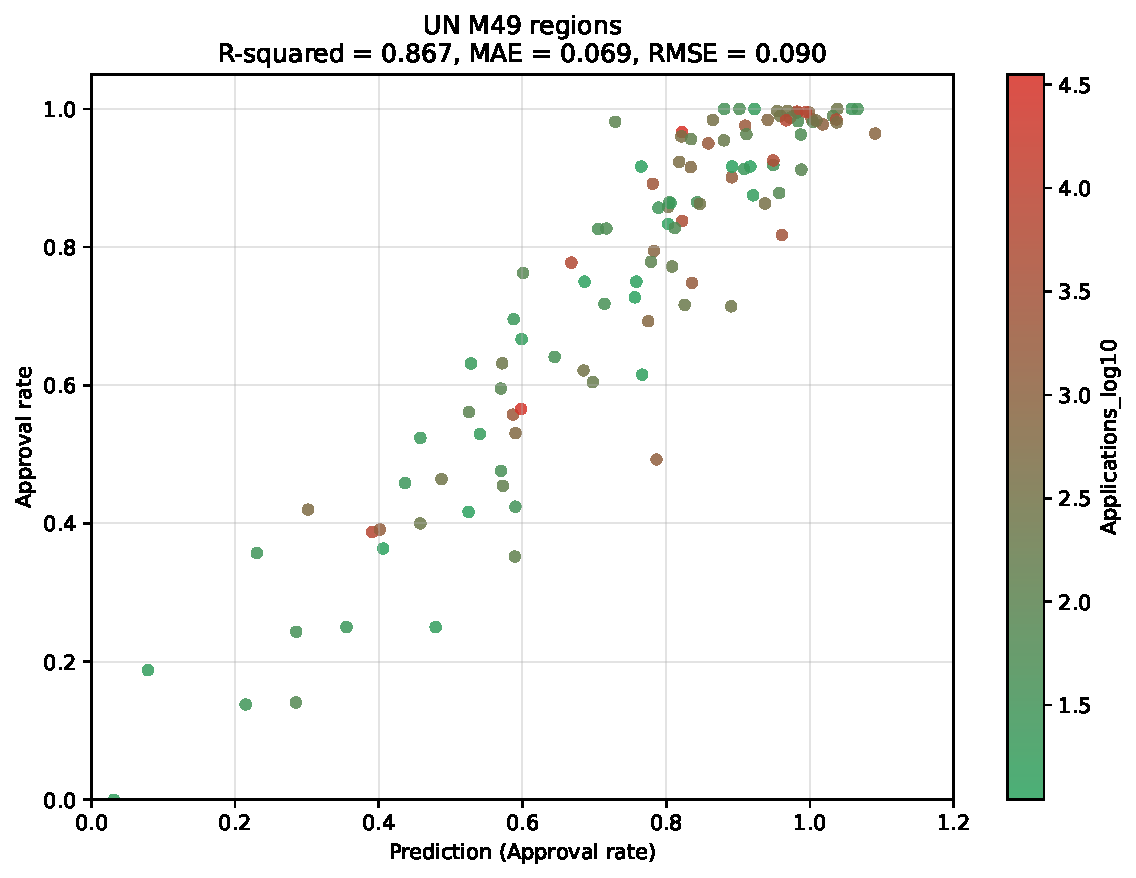
\includegraphics[width=\textwidth]{imgs/approximation_sp_m49.pdf}
\end{minipage}
\hfill
\begin{minipage}{0.48\textwidth}
\centering
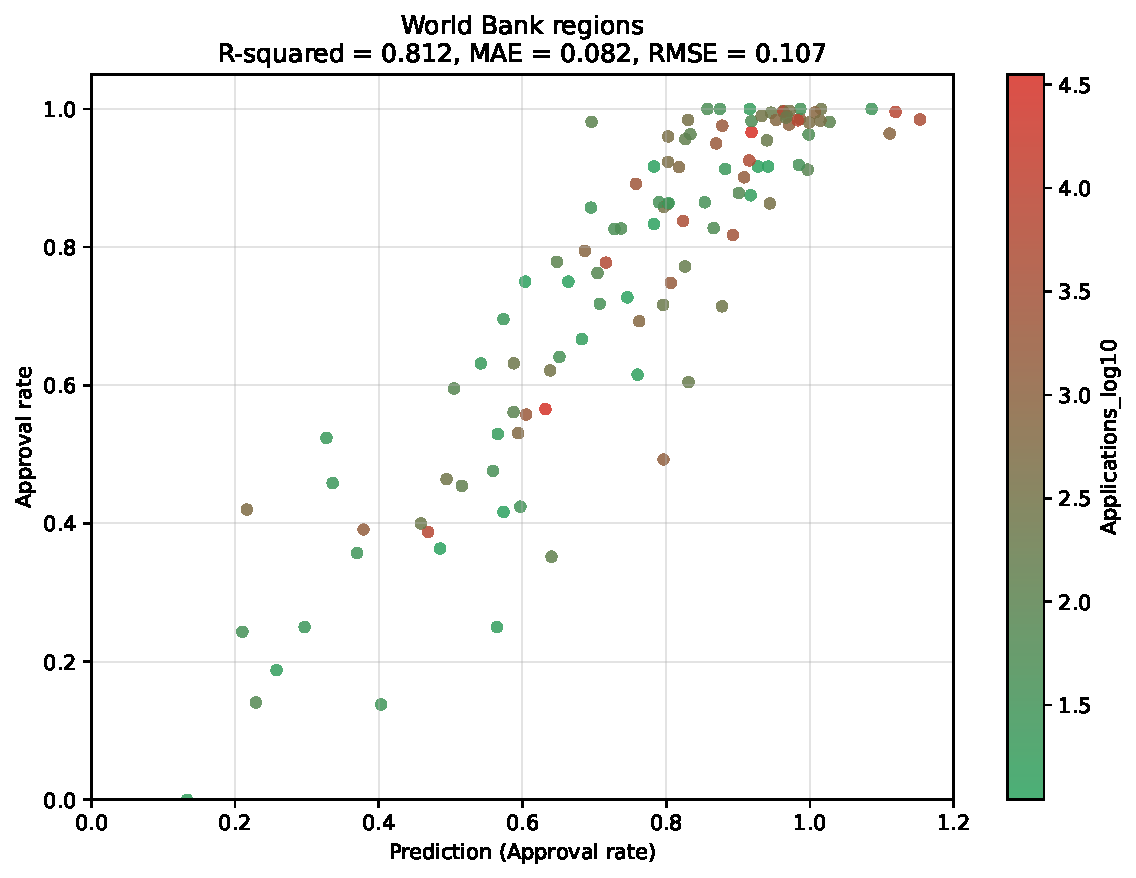
\includegraphics[width=\textwidth]{imgs/approximation_sp_wb.pdf}
\end{minipage}

\vspace{0.7em}

\begin{minipage}{0.48\textwidth}
\centering
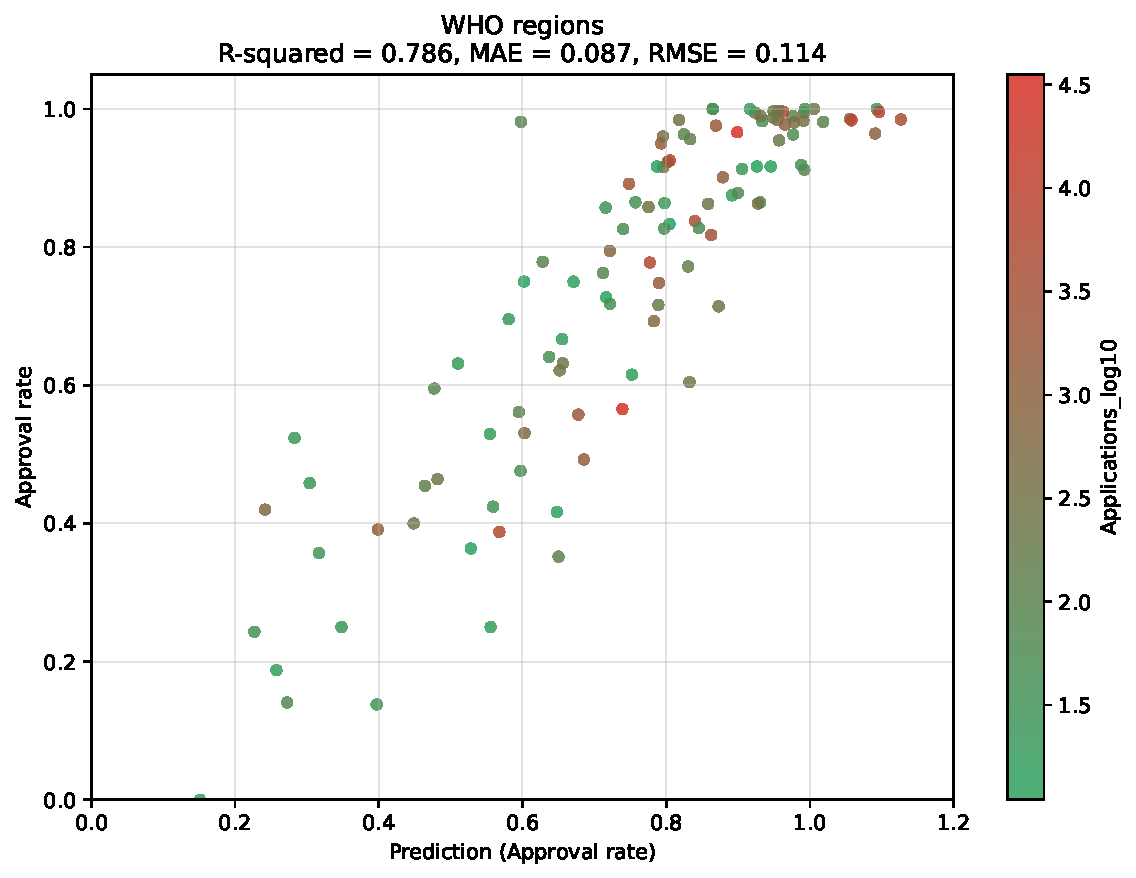
\includegraphics[width=\textwidth]{imgs/approximation_sp_who.pdf}
\end{minipage}
\hfill
\begin{minipage}{0.48\textwidth}
\centering
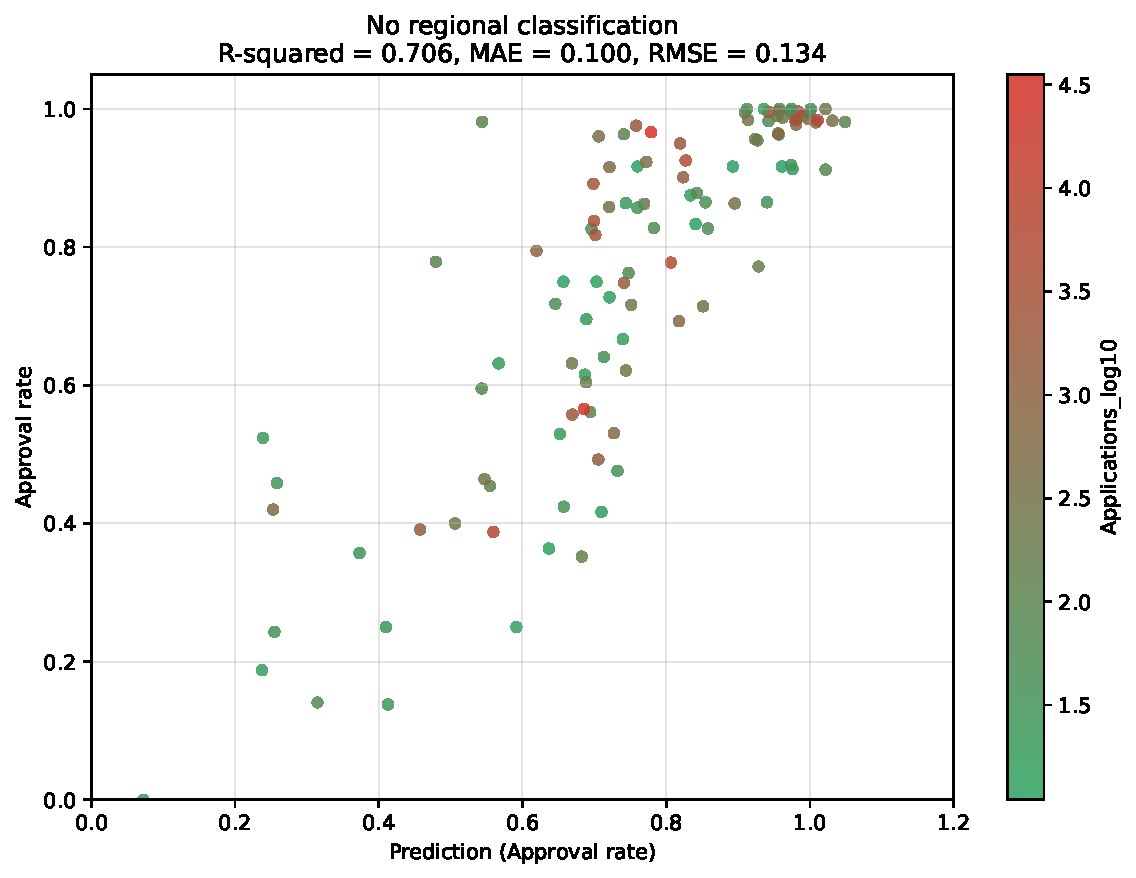
\includegraphics[width=\textwidth]{imgs/approximation_sp_no_region.pdf}
\end{minipage}
\caption{Observed approval rate and fitted approval rate in the four regression specifications: UN M49 regions, World Bank regions, WHO regions, and no regional classification. The plots are generated from \texttt{data/results/approximation\_sp\_m49.svg}, \texttt{data/results/approximation\_sp\_wb.svg}, \texttt{data/results/approximation\_sp\_who.svg}, and \texttt{data/results/approximation\_sp\_no\_region.svg}.}
\label{fig:fitted-observed-approval-rates}
\end{figure}

The plots support the model-comparison results reported above. The UN M49 specification produces the closest visual concentration around the fitted-observed diagonal, while the no-region specification leaves a visibly wider spread. The World Bank and WHO regional specifications fall between these two cases. This pattern is consistent with the score table: regional variables improve fit, and the more detailed UN M49 classification gives the strongest approximation among the current models.

The number of large proportional deviations differs by specification. Table~\ref{tab:large-proportional-deviations} uses the rule that a country is outside the expected band when the observed approval rate is below 80 percent or above 120 percent of the fitted value. The UN M49 model has the fewest such countries, again suggesting that it gives the closest fit among the current specifications.

\begin{table}
\caption{Countries outside the 80--120 percent fitted-value band}
\label{tab:large-proportional-deviations}
\centering
\renewcommand{\arraystretch}{1.2}
\setlength{\tabcolsep}{7pt}
\begin{tabular}{lrrr}
\hline
Specification & Below 80\% & Above 120\% & Total \\
\hline
UN M49 regional model & 10 & 5 & 15 \\
World Bank regional model & 11 & 8 & 19 \\
WHO regional model & 15 & 10 & 25 \\
No-region model & 15 & 13 & 28 \\
\hline
\end{tabular}
\end{table}

Table~\ref{tab:un-m49-large-deviations} lists the countries outside this band in the UN M49 model. These are the countries where the best-fitting current specification still leaves the largest proportional fitted-value deviations.

\begin{table}
\caption{Large proportional deviations in the UN M49 model}
\label{tab:un-m49-large-deviations}
\centering
\renewcommand{\arraystretch}{1.2}
\setlength{\tabcolsep}{6pt}
\begin{tabular}{lrrr}
\hline
Country & Observed & Fitted & Ratio \\
\hline
Chad & 0.000 & 0.032 & 0.000 \\
Afghanistan & 0.141 & 0.285 & 0.495 \\
Uzbekistan & 0.250 & 0.479 & 0.522 \\
Turkey & 0.352 & 0.589 & 0.597 \\
Myanmar & 0.493 & 0.786 & 0.626 \\
Cameroon & 0.138 & 0.215 & 0.642 \\
Yemen & 0.250 & 0.355 & 0.704 \\
Tanzania & 0.424 & 0.590 & 0.719 \\
Algeria & 0.417 & 0.525 & 0.794 \\
Ghana & 0.455 & 0.573 & 0.794 \\
... &  &  &  \\
Kazakhstan & 0.762 & 0.601 & 1.269 \\
Timor Leste & 0.981 & 0.729 & 1.346 \\
Nigeria & 0.420 & 0.302 & 1.392 \\
Sudan & 0.357 & 0.230 & 1.551 \\
Democratic Republic of Congo & 0.188 & 0.079 & 2.375 \\
\hline
\end{tabular}
\end{table}

These cases should not automatically be treated as technical outliers. They show where the current country-level variables and regional classifications do not fit the observed approval rate well. They may point to omitted variables, data quality issues, country-specific applicant composition, policy or processing factors, or other mechanisms not represented in the current dataset.

\section{Robustness or Sensitivity Checks}

The first sensitivity check is already built into the current workflow: the same modelling task is estimated with three alternative regional classifications and with no regional classification. As shown in Table~\ref{tab:model-fit-comparison}, the UN M49 model has the strongest fit, followed by the World Bank regional model, the WHO regional model, and the no-region model. This comparison supports the statement that regional classification matters for model fit and that the more detailed UN M49 classification fits the current data best.

The score tables support the same ordering across several metrics. R-squared declines from 0.867 in the UN M49 model to 0.812 in the World Bank regional model, 0.786 in the WHO regional model, and 0.706 in the no-region model. Mean absolute error and root mean squared error move in the opposite direction: they are smallest in the UN M49 model and largest in the no-region model.

The prediction-rate tables provide a second check. Table~\ref{tab:large-proportional-deviations} shows that the UN M49 model produces the fewest countries outside the 80--120 percent fitted-value band: 15 countries, compared with 19 in the World Bank regional model, 25 in the WHO regional model, and 28 in the no-region model. This supports the view that regional variables improve the fit and that UN M49 is the strongest of the current regional specifications.

The coefficient tables for the UN M49, WHO, World Bank, and no-region specifications are useful for comparing model outputs across alternative specifications. They show whether signs, magnitudes, and statistical significance change across region definitions. However, they do not test all modelling assumptions by themselves.

The coefficient stability summary in Appendix Table~\ref{tab:appendix-coefficient-stability} answers whether the same country-level variables remain important across specifications. It shows two patterns. First, urban population percentage is significant in all four specifications, with negative coefficients and p-values below 0.05. Second, World Bank income-group variables are especially important when UN M49 regions are not used: low-income status and lower-middle-income status are significant in the World Bank, WHO, and no-region models. In the UN M49 model, low-income status is weaker and does not reach the 0.05 threshold ($p = 0.0714$), suggesting that some income-related structure may be absorbed by the more detailed UN M49 regional categories.

The numerical health and development indicators are less stable across specifications. Life expectancy is significant in the UN M49 model ($p = 0.0128$) but not in the World Bank, WHO, or no-region models. WHO DTP3 immunization coverage is significant only in the no-region model ($p = 0.0152$). GDP per capita, GNI per capita, physician density, under-five mortality, maternal mortality, and internet-user percentage do not remain statistically significant in the multivariable coefficient tables, even though several of them have strong bivariate correlations with approval rate. This difference is consistent with overlapping information among country-level development indicators.

This does not mean that these parameters are substantively unimportant. Their bivariate correlations show that they are part of the broader country-level pattern associated with approval rates. In the multivariable models, however, several indicators describe related dimensions of national income, health systems, infrastructure, and institutional development. Once these variables are entered together with income groups and regional classifications, their separate coefficients become harder to distinguish statistically. Their substantive importance is therefore better understood as part of a shared country-level development profile, rather than as isolated independent predictors.

The residual summaries and residuals-versus-fitted plots provide an additional model check. Across all four specifications, mean residuals are 0.0 after rounding, which is expected for these fitted linear models. Table~\ref{tab:residual-summary-by-model} shows that residual spread follows the same ordering as the score tables: the UN M49 model has the smallest residual standard deviation and mean absolute residual, while the no-region model has the largest values. Figure~\ref{fig:residuals-vs-fitted} shows the same comparison graphically. This supports the same conclusion as the score and prediction-rate checks: the UN M49 specification leaves less unexplained error than the alternatives.

\begin{table}
\caption{Residual summary by regression specification}
\label{tab:residual-summary-by-model}
\centering
\renewcommand{\arraystretch}{1.2}
\setlength{\tabcolsep}{6pt}
\begin{tabular}{lrrr}
\hline
Specification & Residual SD & MAE & Max. abs. residual \\
\hline
UN M49 regional model & 0.090 & 0.069 & 0.294 \\
World Bank regional model & 0.108 & 0.082 & 0.314 \\
WHO regional model & 0.115 & 0.087 & 0.384 \\
No-region model & 0.134 & 0.100 & 0.437 \\
\hline
\end{tabular}
\end{table}

\begin{figure}
\centering
\begin{minipage}{0.48\textwidth}
\centering
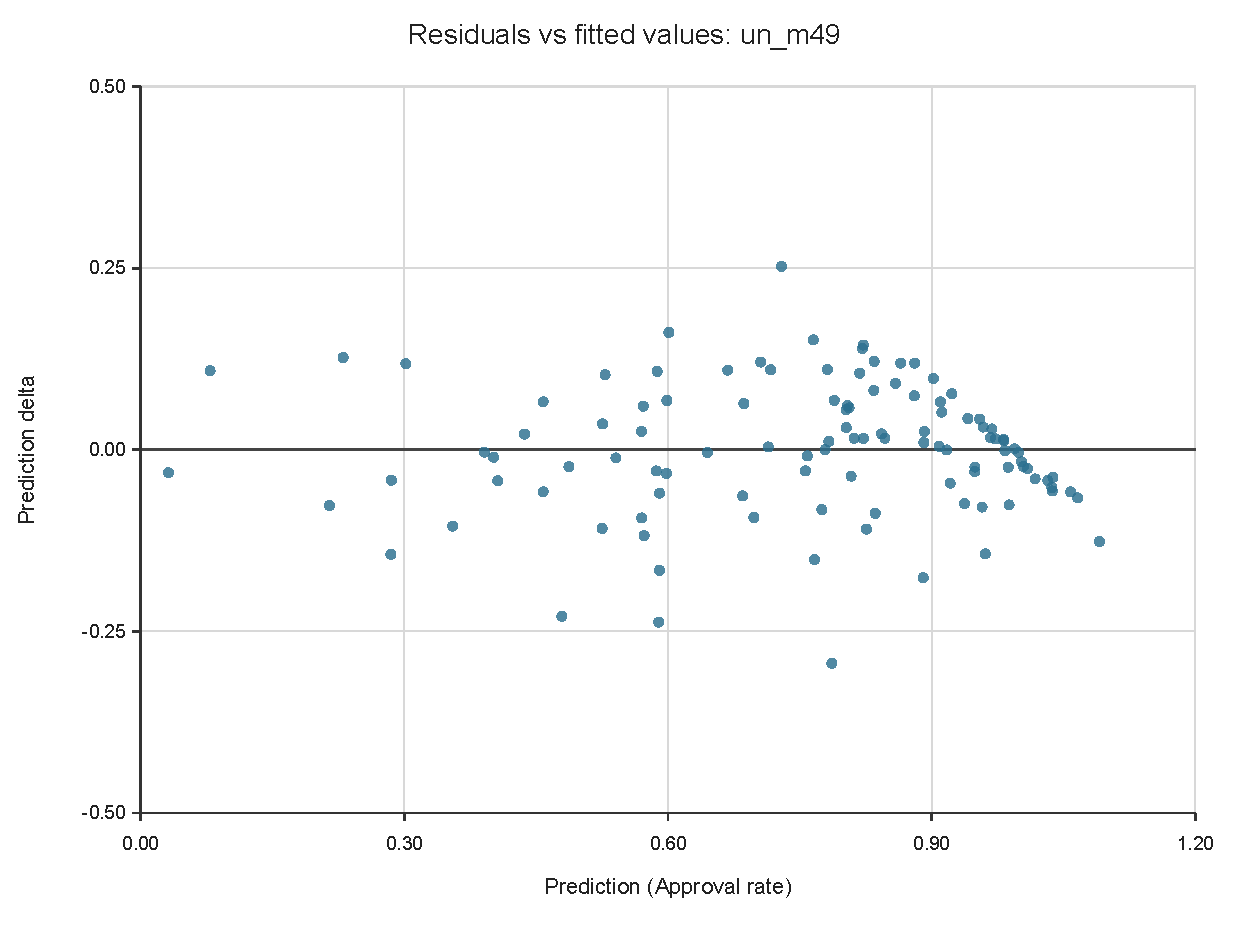
\includegraphics[width=\textwidth]{imgs/residuals_vs_fitted_un_m49.pdf}
\end{minipage}
\hfill
\begin{minipage}{0.48\textwidth}
\centering
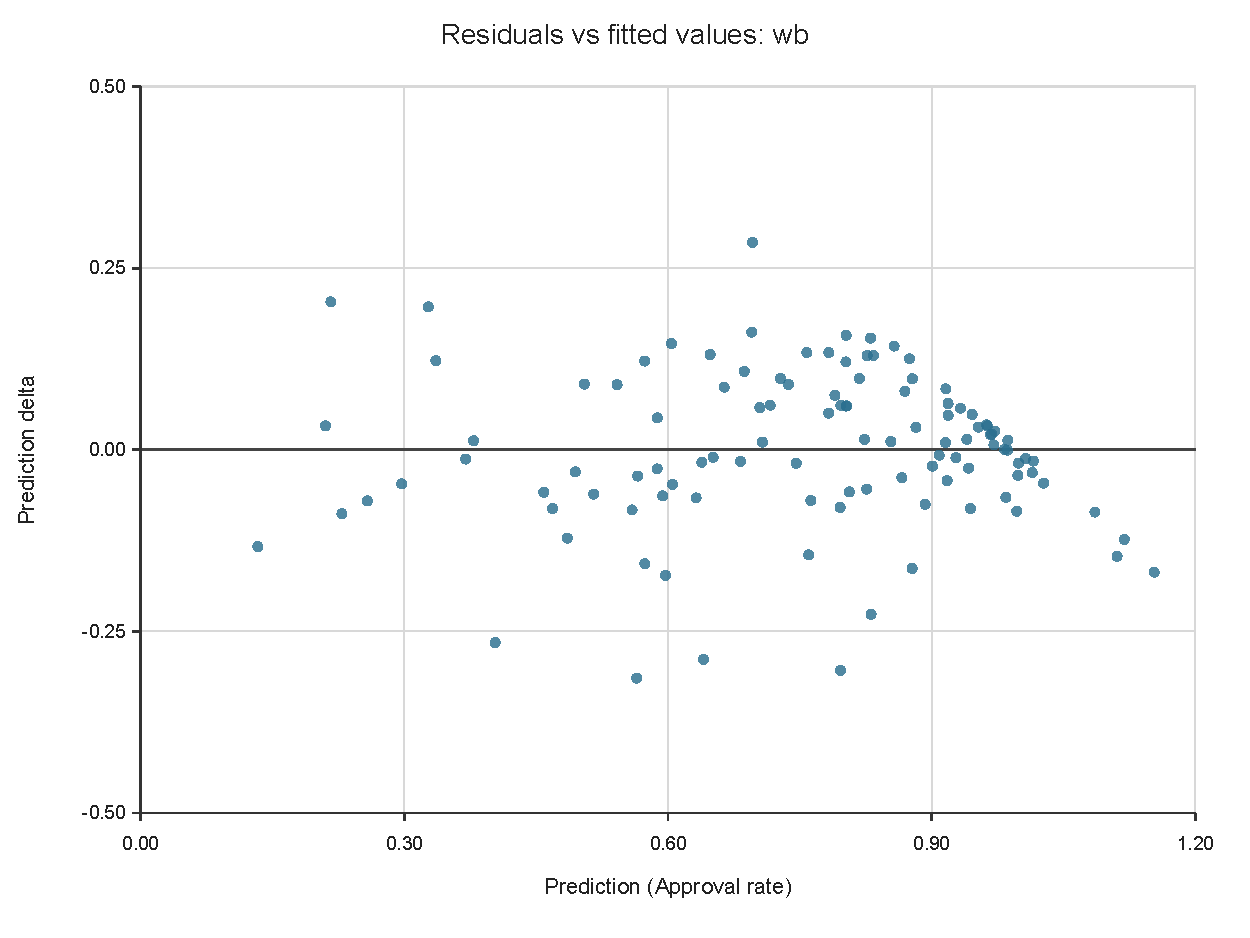
\includegraphics[width=\textwidth]{imgs/residuals_vs_fitted_wb.pdf}
\end{minipage}

\vspace{0.7em}

\begin{minipage}{0.48\textwidth}
\centering
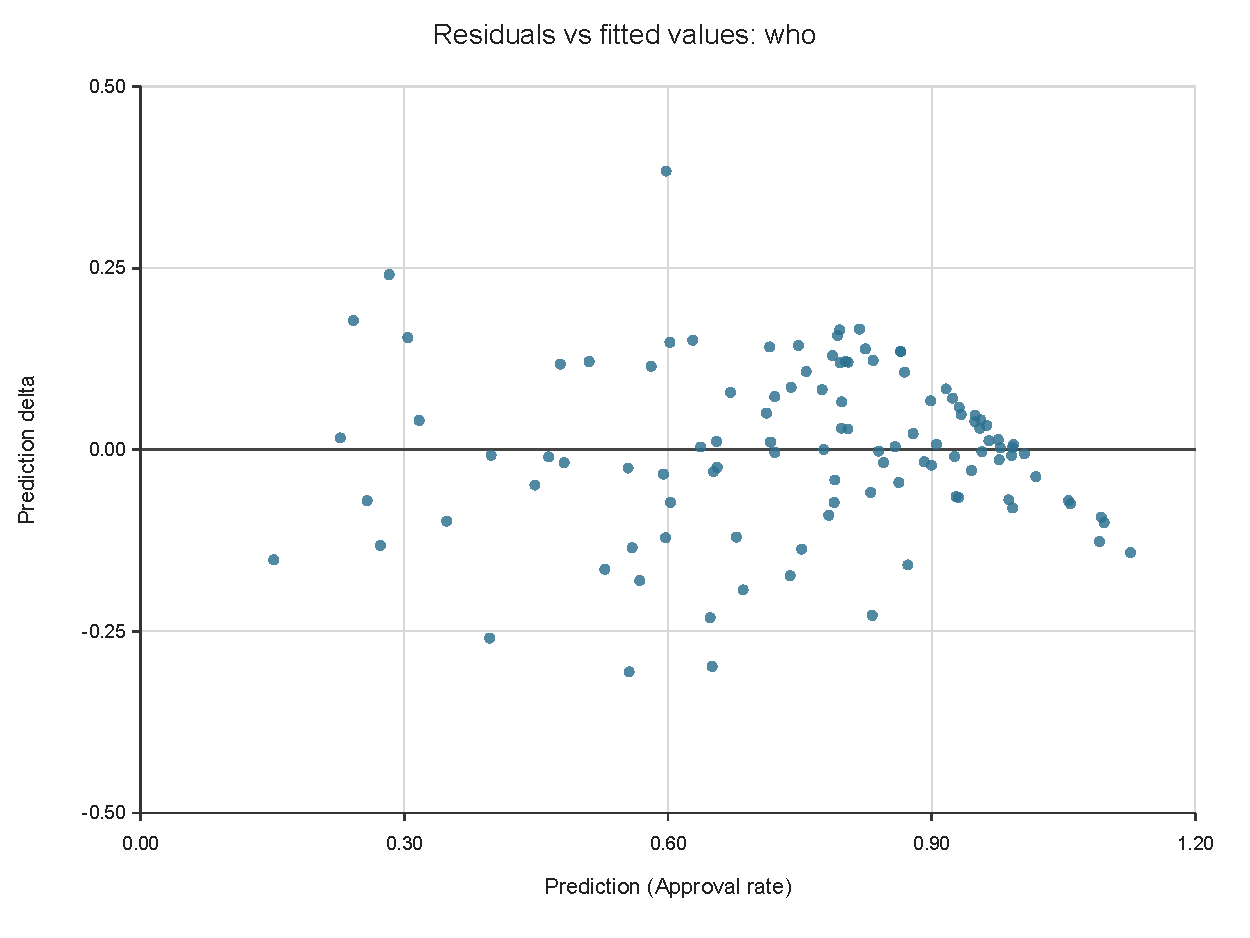
\includegraphics[width=\textwidth]{imgs/residuals_vs_fitted_who.pdf}
\end{minipage}
\hfill
\begin{minipage}{0.48\textwidth}
\centering
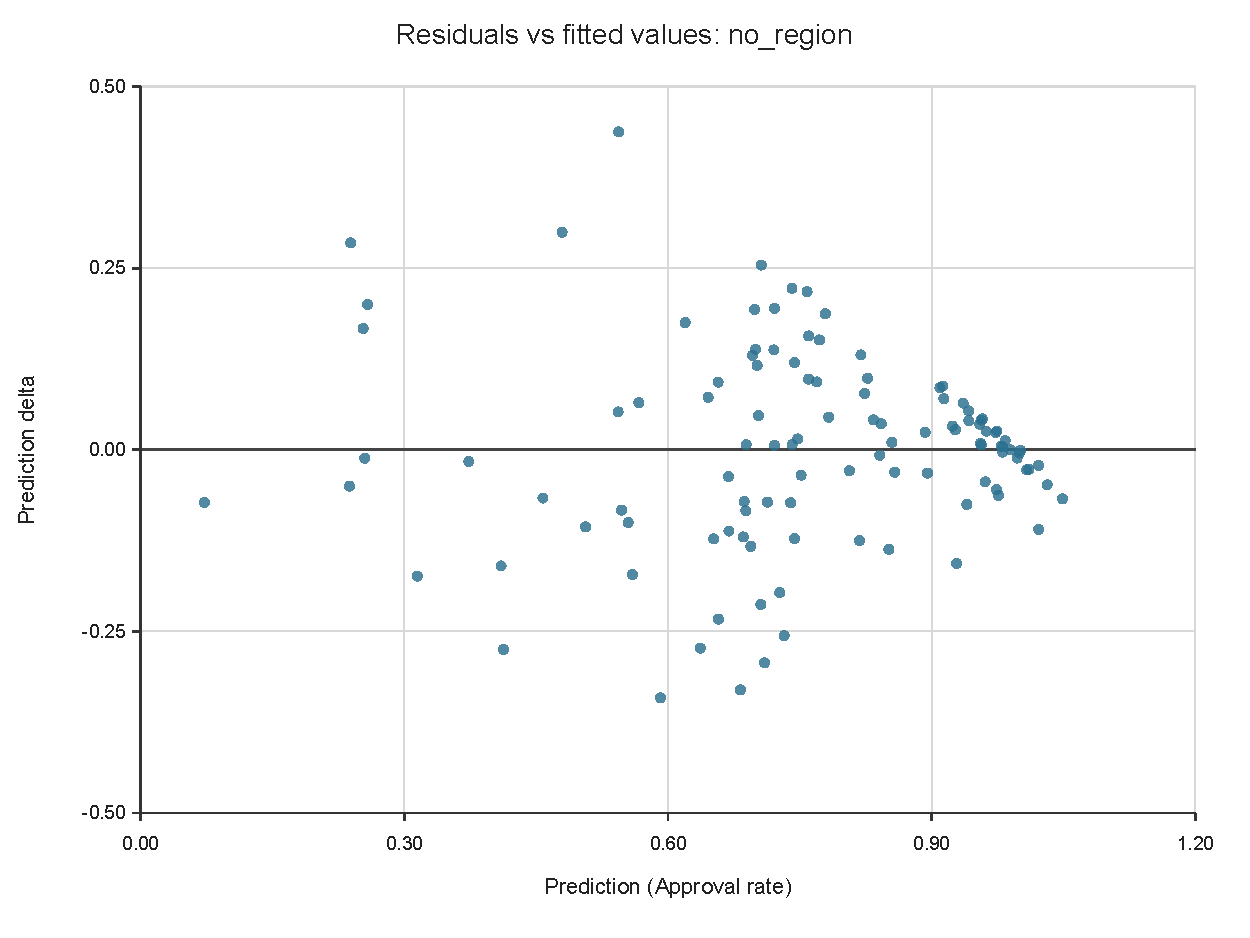
\includegraphics[width=\textwidth]{imgs/residuals_vs_fitted_no_region.pdf}
\end{minipage}
\caption{Residuals against fitted approval rates in the four regression specifications. The figures are generated from \texttt{data/support/residuals\_vs\_fitted\_un\_m49.svg}, \texttt{data/support/residuals\_vs\_fitted\_wb.svg}, \texttt{data/support/residuals\_vs\_fitted\_who.svg}, and \texttt{data/support/residuals\_vs\_fitted\_no\_region.svg}.}
\label{fig:residuals-vs-fitted}
\end{figure}

The largest positive and negative relative residuals are reported in Appendix Tables~\ref{tab:appendix-relative-residuals-positive} and \ref{tab:appendix-relative-residuals-negative}. These tables use \texttt{Prediction\_rate}, the ratio of observed approval rate to fitted approval rate, rather than only the absolute residual. This is useful because the same absolute difference can be more consequential when the fitted approval rate is low. The positive table identifies countries where observed approval is high relative to the fitted value; the negative table identifies countries where observed approval is low relative to the fitted value.

The relative-residual tables also show that several countries recur among the largest positive or negative deviations across model specifications. This supports two interpretations. First, the model comparison is stable enough to support the conclusion that the UN M49 specification has the best fit among the current alternatives. Second, the largest country-level deviations are not explained only by the choice of regional classification. Persistent deviations across specifications may indicate omitted country-specific conditions, applicant-composition differences, documentation or verification factors, or other application-level mechanisms not represented in the current country-level dataset.

An additional weighted UN M49 experiment was estimated in Python using \texttt{Applications\_log10} as the observation weight. This gives more influence to countries with larger log-transformed application volumes while preserving the same UN M49 feature structure. Table~\ref{tab:weighted-un-m49-fit} shows that the weighted model remains close to the unweighted UN M49 model. The mean signed error rounds to 0.0 in all three evaluations. These results indicate that the main UN M49 fit result is stable when countries with larger log-transformed application volumes receive more weight.

\begin{table}
\caption{Weighted UN M49 model fit}
\label{tab:weighted-un-m49-fit}
\centering
\renewcommand{\arraystretch}{1.2}
\setlength{\tabcolsep}{6pt}
\begin{tabular}{lrrr}
\hline
Evaluation & R-squared & MAE & RMSE \\
\hline
Weighted model, weighted metrics & 0.855 & 0.068 & 0.088 \\
Weighted model, unweighted metrics & 0.864 & 0.071 & 0.091 \\
Main UN M49 model, unweighted metrics & 0.867 & 0.069 & 0.090 \\
\hline
\end{tabular}
\end{table}

The weighted coefficient table also supports a cautious interpretation. Table~\ref{tab:weighted-un-m49-significant-terms} shows that life expectancy at birth and urban population percentage remain statistically significant in the weighted UN M49 model. Other variables that were significant in the unweighted UN M49 model, including several regional indicators and the missing World Bank lending-category term, no longer cross the 0.05 threshold. This pattern is substantively plausible. Weighting by application volume reduces the statistical prominence of several regional terms, suggesting that some region-level coefficient patterns in the unweighted model are influenced by treating each country equally regardless of application volume. When countries with more applications receive more weight, the overall UN M49 model fit remains similar, but the evidence for specific regional coefficients becomes weaker. The weighted experiment therefore strengthens the model-fit conclusion while reinforcing caution about individual coefficients.

\begin{table}
\caption{Terms below $p < 0.05$ in the weighted UN M49 specification}
\label{tab:weighted-un-m49-significant-terms}
\centering
\renewcommand{\arraystretch}{1.2}
\setlength{\tabcolsep}{7pt}
\begin{tabular}{lrr}
\hline
Term & Coefficient & $p$ \\
\hline
Life expectancy at birth & 0.543 & 0.0078 \\
Urban population percentage & -0.269 & 0.0051 \\
\hline
\end{tabular}
\end{table}

These checks do not turn the analysis into a causal design. Their role is narrower: to show whether the descriptive model fit and the comparison between regional classifications are stable under reasonable alternative specifications.

\section{Discussion}

The results show that country-level variation in INZ fee-paying student visa approval rates is structured rather than random. Application volume has a positive but limited association with approval rate, as shown in Figure~\ref{fig:applications-log10-approval-rate}. This may reflect application ecosystems that develop around high-volume countries: education agents, advisers, institutional experience, previous successful applicants, and better knowledge of documentary expectations. The present data do not measure these mechanisms directly, so this explanation should be treated as an interpretation rather than a tested cause.

The joined WHO, World Bank, and UN M49 data show that approval rates are also associated with broad country-level conditions. Countries with higher life expectancy, higher internet-use rates, higher physician density, and higher income measures tend to have higher approval rates, while countries with higher mortality indicators tend to have lower approval rates; the strongest bivariate correlations are reported in Table~\ref{tab:approval-country-correlations}. These variables should not be read as direct determinants of individual decisions. They are better understood as indicators of the administrative, economic, health, and institutional context from which applicants prepare evidence for a formal visa process.

The regression results support the same general interpretation. The no-region model already explains a substantial share of the variation, which means that non-region country-level variables contain important information. Adding regional classification improves model fit, and the UN M49 specification performs best among the current alternatives, as shown in Table~\ref{tab:model-fit-comparison} and Figure~\ref{fig:fitted-observed-approval-rates}. This suggests that regional structure matters, but it does not mean that region itself is a causal factor. Regional classifications are summary categories that may capture shared institutional, economic, mobility, documentation, and applicant-composition conditions that are not directly observed in the dataset.

The weighted UN M49 experiment adds an important qualification. When countries with larger log-transformed application volumes receive more weight, the overall model fit remains close to the unweighted UN M49 model, but several regional terms and the missing World Bank lending-category term no longer cross the $p < 0.05$ threshold, as shown in Tables~\ref{tab:weighted-un-m49-fit} and \ref{tab:weighted-un-m49-significant-terms}. This supports the main fit conclusion while reducing confidence in strong interpretations of individual regional coefficients. Some regional patterns are more visible when each country is treated equally, and weaker when high-volume applicant countries receive more influence.

The residual and relative-residual checks show where the current model does not explain observed approval rates well. Positive deviations, where observed approval is higher than fitted approval, may reflect country-specific conditions not captured by the model; these cases are visible in Figure~\ref{fig:residuals-vs-fitted} and Appendix Table~\ref{tab:appendix-relative-residuals-positive}. China is a useful example because it has the largest application volume in the prepared INZ table, with 35,472 applications, but its observed approval rate is still higher than the fitted value in the UN M49 model: 0.966 observed compared with 0.822 fitted, as shown in Appendix Table~\ref{tab:appendix-prediction-comparison}. Possible examples include intergovernmental or inter-educational relationships, established pathways between education providers, scholarship or sponsorship channels, or unusually effective application support structures. Work on China Scholarship Council programmes illustrates how formal scholarship channels and international agreements can structure academic mobility \cite{Xie2025}. These possibilities are not measured in the current data, but they identify plausible directions for further research.

Negative deviations require even more caution. Countries with observed approval rates well below fitted values cannot be explained by the current country-level predictors alone; the largest negative relative residuals are reported in Appendix Table~\ref{tab:appendix-relative-residuals-negative}. These cases may involve applicant-composition differences, programme choice, documentation problems, financial-evidence issues, verification difficulties, or other application-level factors that are absent from the dataset. They should therefore be treated as questions for further empirical investigation, not as evidence for a specific institutional mechanism.

Overall, the analysis supports a narrow conclusion: country-level approval-rate differences are associated with application volume, national development indicators, income categories, and regional classification systems. This conclusion is based on the descriptive application-volume pattern, the bivariate correlations, and the model comparisons reported in Figure~\ref{fig:applications-log10-approval-rate}, Table~\ref{tab:approval-country-correlations}, and Table~\ref{tab:model-fit-comparison}. Within the interpretive framework of this article, these differences are treated as possible evidence of different applicant conditions across countries and regions under the same formal decision framework. The results are useful for describing and modelling variation at the country level, but they do not identify the individual-level reasons why an application is approved or declined.

\section{Limitations}

The analysis is limited by aggregation at the country level. The unit of observation is country or applicant nationality, not an individual application. The models therefore cannot separate applicant-level characteristics, institutional documentation quality, programme choice, education provider characteristics, or officer-level assessment details.

The country-level predictors also overlap substantially. Table~\ref{tab:approval-country-correlations} shows strong pairwise correlations among health, income, internet-use, mortality, and life-expectancy indicators. This supports the substantive interpretation that these variables describe a shared country-level development profile, but it limits interpretation of individual regression coefficients. A full variance inflation factor analysis or other design-matrix diagnostic could examine this more formally, but the present article treats the existing correlation output as sufficient evidence that individual coefficients should be interpreted cautiously.

The results are also sensitive to country matching, missing numerical values, regional classification choices, and the exclusion of countries with fewer than 10 total applications across 2022--2025. Appendix Table~\ref{tab:appendix-excluded-countries} reports the excluded countries, and Table~\ref{tab:regional-classification-counts} reports the regional classification alternatives used in the model comparison. The comparison across UN M49, World Bank, WHO, and no-region specifications addresses part of this sensitivity, but it does not remove the broader limitations of observational, aggregated data.

\section{Conclusion}

This article shows that country-level variation in Immigration New Zealand fee-paying student visa approval rates during 2022--2025 is associated with application volume, country-level development indicators, income categories, and regional classification systems. The strongest current model fit is obtained with the UN M49 regional specification, as reported in Table~\ref{tab:model-fit-comparison}, but the results also show that non-region country-level variables carry substantial explanatory information. The analysis should therefore be read as a country-level descriptive and modelling exercise, not as a causal account of individual visa decisions or as evidence about officer-level assessment behaviour.

The main empirical contribution is to connect INZ student visa decision outcomes with external country-level reference data in a reproducible workflow. This makes visible both broad structure and unexplained country-specific deviations. The broad structure is summarized in Tables~\ref{tab:approval-country-correlations} and \ref{tab:model-fit-comparison}; the deviations are summarized in Tables~\ref{tab:large-proportional-deviations} and \ref{tab:un-m49-large-deviations}. Together, these outputs support cautious interpretation of country-level application conditions and identify where the current data are insufficient and where more detailed research is needed.

It is difficult to assume that WHO and World Bank indicators directly influence visa approval rates. A more cautious interpretation is that these indicators mark broader country-specific conditions that are not directly observed in the present dataset, consistent with the correlation and coefficient-stability results in Tables~\ref{tab:approval-country-correlations} and \ref{tab:appendix-coefficient-stability}. Such hidden conditions may influence both the measured WHO and World Bank variables and the practical circumstances under which applicants prepare visa evidence. Identifying these country-specific mechanisms is therefore a central task for further research.

Future work should extend the comparison beyond New Zealand by examining student visa decisions in other receiving countries, especially where approval, refusal, enrolment, or policy-restrictiveness data can be linked over time. Studies of the United States and Canada show that visa restrictiveness and approval patterns can affect international student enrolment and mobility \cite{Chen2023,Gonnot2025}. A comparative design would therefore help distinguish patterns that are specific to INZ from broader features of student visa systems in destination countries.

Further models should add country-level variables suggested by the student-mobility literature, provided that their definitions and provenance are clear. Relevant candidates include passport or visa-access measures linked to the global mobility divide \cite{Shachar2014,Neumayer2006,Mau2015,Gulel2025}; language, geographic distance, existing student or migrant networks, institutional quality, political freedom, fees, and origin- or destination-country economic conditions \cite{PerkinsNeumayer2014,Abbott2016,Bessey2012}; and formal education or development channels such as foreign aid projects, scholarship programmes, and structured inter-country education relationships \cite{LanatiThiele2020,Xie2025}. These variables would test whether the countries with approval rates above or below the fitted values, reported in Tables~\ref{tab:un-m49-large-deviations}, \ref{tab:appendix-relative-residuals-positive}, and \ref{tab:appendix-relative-residuals-negative}, are associated with documented mobility channels, application-support structures, or information conditions rather than with region or development indicators alone.

To inform our empirical analysis, we propose a basic theoretical model to understand how incomplete information affects the processing of visa applications by immigration officers.

\section{Appendices or Supplementary Material}

The appendix tables and figures refer to repository-relative files in the project repository \cite{KaplanINZRepo}.

\subsection{Student Visa Application Preparation}
\label{app:student-visa-preparation}

The INZ student visa decision data are useful for this analysis partly because a fee-paying student visa application is unlikely to be a casual or spontaneous action. Before an application can be assessed, the applicant normally has to assemble educational, financial, personal, health, and documentary evidence. This does not prove that every application is strong, complete, or equally supported. It does mean that the published decision records represent applications that passed through a substantial preparation process before reaching a formal decision.

\begin{table}
\caption{Typical preparation requirements before a fee-paying student visa decision}
\label{tab:appendix-student-visa-preparation}
\centering
\renewcommand{\arraystretch}{1.2}
\setlength{\tabcolsep}{6pt}
\begin{tabular}{p{0.28\textwidth}p{0.58\textwidth}}
\hline
Preparation area & Examples of required or commonly relevant evidence \\
\hline
Education pathway & Identifying an education provider, submitting documents to that provider, receiving an offer of place, and documenting previous education. \\
Tuition and insurance & Paying tuition or documenting tuition arrangements, receiving confirmation from the education provider, and arranging medical or travel insurance where required. \\
Financial capacity & Providing bank statements or other evidence of funds for study and living costs, together with explanations of source of funds and relevant incoming transfers. \\
Personal and travel history & Providing previous education and work history, explaining gaps in education or employment, and documenting travel history where requested. \\
Health and character & Providing relevant health information, medical examination material where required, and character-related information required by the visa process. \\
Home-country ties and translations & Documenting family relationships, property or other ties where relevant, and providing certified translations for documents not originally in English. \\
\hline
\end{tabular}
\end{table}

This preparation burden matters for interpretation. The observed INZ application counts are not treated as a simple measure of abstract interest in New Zealand study. They are better understood as counts of completed applications that were submitted after applicants had already undertaken a costly and document-intensive process. For this reason, variation in approval rates may reflect differences in the practical conditions under which applicants can assemble convincing evidence, not only differences in demand for study.

\subsection{Countries Excluded Before Regression}

Table~\ref{tab:appendix-excluded-countries} reports countries present in the aggregated INZ decision data but not retained in the final regression table. Eight countries were not retained after the reference-data join or missing-value filter. The remaining countries were excluded because they had fewer than 10 total applications across 2022--2025.

{\scriptsize
\renewcommand{\arraystretch}{1.12}
\setlength{\tabcolsep}{5pt}
\begin{longtable}{p{0.28\textwidth}rrp{0.36\textwidth}}
\caption{Countries excluded before regression modelling}\label{tab:appendix-excluded-countries}\\
\hline
Country & Applications & Approval rate & Exclusion reason \\
\hline
\endfirsthead
\multicolumn{4}{l}{\tablename\ \thetable{} -- continued from previous page}\\
\hline
Country & Applications & Approval rate & Exclusion reason \\
\hline
\endhead
Hong Kong & 1397 & 0.981 & Not retained after reference join or missing-value filter \\
Taiwan & 1094 & 0.976 & Not retained after reference join or missing-value filter \\
Macau & 69 & 0.928 & Not retained after reference join or missing-value filter \\
Tuvalu & 59 & 0.983 & Not retained after reference join or missing-value filter \\
Palestine & 15 & 0.533 & Not retained after reference join or missing-value filter \\
Lithuania & 10 & 0.900 & Not retained after reference join or missing-value filter \\
Malawi & 10 & 0.600 & Not retained after reference join or missing-value filter \\
Trinidad and Tobago & 10 & 0.800 & Not retained after reference join or missing-value filter \\
Iceland & 9 & 1.000 & Fewer than 10 total applications \\
Liberia & 9 & 0.000 & Fewer than 10 total applications \\
Namibia & 9 & 0.556 & Fewer than 10 total applications \\
Guatemala & 8 & 0.750 & Fewer than 10 total applications \\
Nauru & 8 & 1.000 & Fewer than 10 total applications \\
Albania & 7 & 0.714 & Fewer than 10 total applications \\
Benin & 7 & 0.286 & Fewer than 10 total applications \\
Estonia & 7 & 1.000 & Fewer than 10 total applications \\
Georgia & 7 & 0.571 & Fewer than 10 total applications \\
Croatia & 6 & 1.000 & Fewer than 10 total applications \\
El Salvador & 6 & 1.000 & Fewer than 10 total applications \\
Guyana & 6 & 0.833 & Fewer than 10 total applications \\
Marshall Islands & 6 & 1.000 & Fewer than 10 total applications \\
South Sudan & 6 & 0.333 & Fewer than 10 total applications \\
St Lucia & 6 & 1.000 & Fewer than 10 total applications \\
Azerbaijan & 5 & 0.800 & Fewer than 10 total applications \\
Gambia & 5 & 0.200 & Fewer than 10 total applications \\
Haiti & 5 & 0.200 & Fewer than 10 total applications \\
Mozambique & 5 & 0.800 & Fewer than 10 total applications \\
Palau & 5 & 1.000 & Fewer than 10 total applications \\
Suriname & 5 & 1.000 & Fewer than 10 total applications \\
Swaziland & 5 & 0.800 & Fewer than 10 total applications \\
Tunisia & 5 & 0.400 & Fewer than 10 total applications \\
Armenia & 4 & 0.500 & Fewer than 10 total applications \\
Bahrain & 4 & 1.000 & Fewer than 10 total applications \\
Belize & 4 & 1.000 & Fewer than 10 total applications \\
Burundi & 4 & 0.000 & Fewer than 10 total applications \\
Eritrea & 4 & 0.750 & Fewer than 10 total applications \\
Grenada & 4 & 0.750 & Fewer than 10 total applications \\
Macedonia & 4 & 1.000 & Fewer than 10 total applications \\
Mali & 4 & 0.750 & Fewer than 10 total applications \\
Moldova & 4 & 0.750 & Fewer than 10 total applications \\
Serbia & 4 & 0.750 & Fewer than 10 total applications \\
Sierra Leone & 4 & 0.000 & Fewer than 10 total applications \\
Angola & 3 & 0.000 & Fewer than 10 total applications \\
Barbados & 3 & 1.000 & Fewer than 10 total applications \\
Congo & 3 & 0.000 & Fewer than 10 total applications \\
Dominica & 3 & 0.667 & Fewer than 10 total applications \\
Federated States of Micronesia & 3 & 1.000 & Fewer than 10 total applications \\
Liechtenstein & 3 & 1.000 & Fewer than 10 total applications \\
Malta & 3 & 1.000 & Fewer than 10 total applications \\
Slovenia & 3 & 1.000 & Fewer than 10 total applications \\
Somalia & 3 & 0.000 & Fewer than 10 total applications \\
St Kitts - Nevis & 3 & 0.667 & Fewer than 10 total applications \\
St Vincent and the Grenadines & 3 & 1.000 & Fewer than 10 total applications \\
Tajikistan & 3 & 0.667 & Fewer than 10 total applications \\
Australia & 2 & 1.000 & Fewer than 10 total applications \\
Bermuda & 2 & 0.500 & Fewer than 10 total applications \\
Guinea & 2 & 0.000 & Fewer than 10 total applications \\
Senegal & 2 & 0.000 & Fewer than 10 total applications \\
Seychelles & 2 & 1.000 & Fewer than 10 total applications \\
Bahamas & 1 & 1.000 & Fewer than 10 total applications \\
Bosnia \& Herzegovina & 1 & 1.000 & Fewer than 10 total applications \\
Cape Verde & 1 & 1.000 & Fewer than 10 total applications \\
Cuba & 1 & 1.000 & Fewer than 10 total applications \\
Djibouti & 1 & 0.000 & Fewer than 10 total applications \\
Madagascar & 1 & 0.000 & Fewer than 10 total applications \\
Nicaragua & 1 & 1.000 & Fewer than 10 total applications \\
Niger & 1 & 0.000 & Fewer than 10 total applications \\
North Korea & 1 & 0.000 & Fewer than 10 total applications \\
Togo & 1 & 0.000 & Fewer than 10 total applications \\
\hline
\end{longtable}
}

The following tables report the full coefficient and p-value outputs for the four regression specifications discussed in Section~5.3. The source files are \texttt{data/results/Coefficients\_un\_m49.csv}, \texttt{data/results/Coefficients\_wb.csv}, \texttt{data/results/Coefficients\_who.csv}, and \texttt{data/results/Coefficients\_no\_region.csv}.

{\scriptsize
\renewcommand{\arraystretch}{1.15}
\setlength{\tabcolsep}{8pt}
\begin{longtable}{p{0.58\textwidth}r@{\hspace{1.5em}}r}
\caption{Full coefficient table for the UN M49 regional specification}\label{tab:appendix-coefficients-un-m49}\\
\hline
Term & Coefficient & $p$ \\
\hline
\endfirsthead
\multicolumn{3}{l}{\tablename\ \thetable{} -- continued from previous page}\\
\hline
Term & Coefficient & $p$ \\
\hline
\endhead
Urban\_population\_pct & -0.2795 & 0.0053 \\
UN M49=Northern Africa & -0.2537 & 0.0109 \\
Life\_expectancy\_at\_birth\_years & 0.4992 & 0.0128 \\
WB\_FY2026\_Lending\_Category=Missing & 0.2425 & 0.0156 \\
UN M49=Middle Africa & -0.2749 & 0.0219 \\
UN M49=Southern Asia & -0.2100 & 0.0336 \\
Intercept & 0.4674 & 0.0492 \\
WB\_FY2026\_Income\_Group=Low income & -0.1980 & 0.0714 \\
UN M49=Melanesia & 0.2055 & 0.0861 \\
UN M49=Central Asia & -0.1989 & 0.0902 \\
UN M49=Western Asia & -0.1674 & 0.0904 \\
WB\_FY2026\_Lending\_Category=IBRD & 0.1036 & 0.1439 \\
UN M49=South-eastern Asia & 0.1074 & 0.2368 \\
WB\_FY2026\_Lending\_Category=IDA & 0.0600 & 0.3012 \\
UN M49=Micronesia & 0.1634 & 0.3124 \\
Internet\_users\_pct\_population & 0.1136 & 0.3553 \\
UN M49=Southern Europe & -0.0925 & 0.4785 \\
UN M49=Polynesia & 0.0970 & 0.4848 \\
GDP\_per\_capita\_current\_USD & -0.1922 & 0.4888 \\
UN M49=Northern Europe & -0.0755 & 0.5001 \\
GNI\_per\_capita\_Atlas\_current\_USD & 0.1768 & 0.5223 \\
UN M49=Central America & 0.0613 & 0.5712 \\
WB\_FY2026\_Income\_Group=Lower middle income & -0.0389 & 0.5992 \\
UN M49=Eastern Africa & -0.0478 & 0.6506 \\
UN M49=South America & 0.0438 & 0.6554 \\
WHO\_DTP3\_Immunization\_Coverage\_pct & -0.0355 & 0.6678 \\
UN M49=Western Europe & -0.0315 & 0.7865 \\
WB\_FY2026\_Income\_Group=Missing & -0.0290 & 0.7943 \\
UN M49=Northern America & -0.0335 & 0.7951 \\
WB\_FY2026\_Income\_Group=Upper middle income & -0.0148 & 0.7967 \\
UN M49=Eastern Asia & -0.0261 & 0.8053 \\
UN M49=Eastern Europe & 0.0192 & 0.8582 \\
UN M49=Southern Africa & 0.0204 & 0.8628 \\
WHO\_Physician\_Density\_per\_10000\_population & -0.0140 & 0.9018 \\
WHO\_Under5\_Mortality\_per\_1000\_live\_births & 0.0245 & 0.9164 \\
UN M49=Western Africa & -0.0105 & 0.9384 \\
WHO\_Maternal\_Mortality\_per\_100000\_live\_births & -0.0081 & 0.9689 \\
\hline
\end{longtable}

\begin{longtable}{p{0.58\textwidth}r@{\hspace{1.5em}}r}
\caption{Full coefficient table for the World Bank regional specification}\label{tab:appendix-coefficients-wb}\\
\hline
Term & Coefficient & $p$ \\
\hline
\endfirsthead
\multicolumn{3}{l}{\tablename\ \thetable{} -- continued from previous page}\\
\hline
Term & Coefficient & $p$ \\
\hline
\endhead
WB\_FY2026\_Region=Middle East, North Africa, Afghanistan \& Pakistan & -0.2695 & $8.194e{-8}$ \\
Intercept & 0.9166 & $5.844e{-7}$ \\
WB\_FY2026\_Income\_Group=Low income & -0.4067 & $5.477e{-5}$ \\
WB\_FY2026\_Region=Europe \& Central Asia & -0.1846 & $3.689e{-4}$ \\
WB\_FY2026\_Region=South Asia & -0.2322 & $5.548e{-4}$ \\
WB\_FY2026\_Region=Sub-Saharan Africa & -0.1561 & 0.0042 \\
Urban\_population\_pct & -0.2545 & 0.0061 \\
WB\_FY2026\_Lending\_Category=Missing & 0.2244 & 0.0171 \\
WB\_FY2026\_Income\_Group=Lower middle income & -0.1355 & 0.0461 \\
WB\_FY2026\_Income\_Group=Upper middle income & -0.0914 & 0.0889 \\
WB\_FY2026\_Lending\_Category=IBRD & 0.1114 & 0.0918 \\
WB\_FY2026\_Region=North America & -0.1633 & 0.1001 \\
Life\_expectancy\_at\_birth\_years & 0.2595 & 0.1672 \\
WB\_FY2026\_Region=Latin America \& Caribbean & -0.0644 & 0.2041 \\
WHO\_DTP3\_Immunization\_Coverage\_pct & -0.0970 & 0.2097 \\
WB\_FY2026\_Lending\_Category=IDA & 0.0692 & 0.2267 \\
WB\_FY2026\_Income\_Group=Missing & -0.1243 & 0.2511 \\
WHO\_Under5\_Mortality\_per\_1000\_live\_births & -0.1944 & 0.3301 \\
GNI\_per\_capita\_Atlas\_current\_USD & 0.1541 & 0.5663 \\
GDP\_per\_capita\_current\_USD & -0.1087 & 0.7076 \\
Internet\_users\_pct\_population & 0.0271 & 0.7942 \\
WHO\_Maternal\_Mortality\_per\_100000\_live\_births & -0.0367 & 0.8419 \\
WHO\_Physician\_Density\_per\_10000\_population & -0.0041 & 0.9680 \\
\hline
\end{longtable}

\begin{longtable}{p{0.58\textwidth}r@{\hspace{1.5em}}r}
\caption{Full coefficient table for the WHO regional specification}\label{tab:appendix-coefficients-who}\\
\hline
Term & Coefficient & $p$ \\
\hline
\endfirsthead
\multicolumn{3}{l}{\tablename\ \thetable{} -- continued from previous page}\\
\hline
Term & Coefficient & $p$ \\
\hline
\endhead
Intercept & 0.8794 & $3.670e{-6}$ \\
WB\_FY2026\_Income\_Group=Low income & -0.4423 & $4.232e{-5}$ \\
WHO\_Region=Western Pacific Region & 0.1980 & $9.745e{-4}$ \\
WB\_FY2026\_Income\_Group=Lower middle income & -0.1780 & 0.0127 \\
Urban\_population\_pct & -0.2370 & 0.0132 \\
WB\_FY2026\_Lending\_Category=Missing & 0.2311 & 0.0198 \\
WB\_FY2026\_Income\_Group=Upper middle income & -0.1039 & 0.0680 \\
WHO\_Region=Region of the Americas & 0.1219 & 0.0691 \\
WB\_FY2026\_Lending\_Category=IBRD & 0.1173 & 0.0952 \\
WHO\_DTP3\_Immunization\_Coverage\_pct & -0.1333 & 0.1146 \\
WHO\_Region=South-East Asia Region & 0.0849 & 0.1933 \\
WB\_FY2026\_Income\_Group=Missing & -0.1484 & 0.1958 \\
WHO\_Under5\_Mortality\_per\_1000\_live\_births & -0.2102 & 0.3220 \\
WHO\_Region=Eastern Mediterranean Region & -0.0545 & 0.3817 \\
WB\_FY2026\_Lending\_Category=IDA & 0.0481 & 0.4213 \\
Life\_expectancy\_at\_birth\_years & 0.1354 & 0.4701 \\
GNI\_per\_capita\_Atlas\_current\_USD & 0.1327 & 0.6318 \\
WHO\_Region=European Region & 0.0319 & 0.6626 \\
WHO\_Physician\_Density\_per\_10000\_population & -0.0393 & 0.7146 \\
GDP\_per\_capita\_current\_USD & -0.0843 & 0.7816 \\
WHO\_Maternal\_Mortality\_per\_100000\_live\_births & -0.0494 & 0.7995 \\
Internet\_users\_pct\_population & -0.0107 & 0.9230 \\
\hline
\end{longtable}

\begin{longtable}{p{0.58\textwidth}r@{\hspace{1.5em}}r}
\caption{Full coefficient table for the no-region specification}\label{tab:appendix-coefficients-no-region}\\
\hline
Term & Coefficient & $p$ \\
\hline
\endfirsthead
\multicolumn{3}{l}{\tablename\ \thetable{} -- continued from previous page}\\
\hline
Term & Coefficient & $p$ \\
\hline
\endhead
Intercept & 1.1160 & $3.208e{-8}$ \\
WB\_FY2026\_Income\_Group=Low income & -0.6087 & $2.500e{-7}$ \\
WB\_FY2026\_Income\_Group=Lower middle income & -0.2242 & 0.0047 \\
Urban\_population\_pct & -0.2635 & 0.0081 \\
WHO\_DTP3\_Immunization\_Coverage\_pct & -0.2036 & 0.0152 \\
WHO\_Under5\_Mortality\_per\_1000\_live\_births & -0.4155 & 0.0758 \\
WB\_FY2026\_Income\_Group=Upper middle income & -0.1059 & 0.0958 \\
WB\_FY2026\_Income\_Group=Missing & -0.2087 & 0.1085 \\
WB\_FY2026\_Lending\_Category=Missing & 0.1644 & 0.1301 \\
WB\_FY2026\_Lending\_Category=IDA & 0.0833 & 0.2166 \\
WB\_FY2026\_Lending\_Category=IBRD & 0.0930 & 0.2363 \\
WHO\_Physician\_Density\_per\_10000\_population & -0.1130 & 0.2560 \\
GNI\_per\_capita\_Atlas\_current\_USD & 0.2416 & 0.4372 \\
Life\_expectancy\_at\_birth\_years & 0.0871 & 0.6543 \\
GDP\_per\_capita\_current\_USD & -0.1465 & 0.6644 \\
Internet\_users\_pct\_population & 0.0134 & 0.9087 \\
WHO\_Maternal\_Mortality\_per\_100000\_live\_births & 0.0182 & 0.9329 \\
\hline
\end{longtable}
}

\subsection{Coefficient Stability Summary}

Table~\ref{tab:appendix-coefficient-stability} reports the cross-specification coefficient stability summary from \texttt{data/support/Coefficients\_stability\_summary.csv}. The table gives the number of model specifications in which each term appears, the number of those specifications where $p < 0.05$, and the minimum and maximum p-values observed across the specifications where the term is present.

{\tiny
\renewcommand{\arraystretch}{1.12}
\setlength{\tabcolsep}{2pt}
\begin{longtable}{p{0.38\textwidth}p{0.08\textwidth}rr@{\hspace{0.7em}}rrp{0.15\textwidth}}
\caption{Coefficient stability summary across regression specifications}\label{tab:appendix-coefficient-stability}\\
\hline
Term & Type & Models & Sig. & Min. $p$ & Max. $p$ & Stability \\
\hline
\endfirsthead
\multicolumn{7}{l}{\tablename\ \thetable{} -- continued from previous page}\\
\hline
Term & Type & Models & Sig. & Min. $p$ & Max. $p$ & Stability \\
\hline
\endhead
Urban\_population\_pct & Variable & 4 & 4 & 0.0053 & 0.0132 & stable significant \\
WB\_FY2026\_Income\_Group=Low income & Variable & 4 & 3 & $2.500e{-7}$ & 0.0714 & partly stable \\
WB\_FY2026\_Income\_Group=Lower middle income & Variable & 4 & 3 & 0.0047 & 0.5992 & partly stable \\
WB\_FY2026\_Lending\_Category=Missing & Variable & 4 & 3 & 0.0156 & 0.1301 & partly stable \\
Life\_expectancy\_at\_birth\_years & Variable & 4 & 1 & 0.0128 & 0.6543 & specification dependent \\
WHO\_DTP3\_Immunization\_Coverage\_pct & Variable & 4 & 1 & 0.0152 & 0.6678 & specification dependent \\
WB\_FY2026\_Income\_Group=Upper middle income & Variable & 4 & 0 & 0.0680 & 0.7967 & not significant \\
WHO\_Under5\_Mortality\_per\_1000\_live\_births & Variable & 4 & 0 & 0.0758 & 0.9164 & not significant \\
WB\_FY2026\_Lending\_Category=IBRD & Variable & 4 & 0 & 0.0918 & 0.2363 & not significant \\
WB\_FY2026\_Income\_Group=Missing & Variable & 4 & 0 & 0.1085 & 0.7943 & not significant \\
WB\_FY2026\_Lending\_Category=IDA & Variable & 4 & 0 & 0.2166 & 0.4213 & not significant \\
WHO\_Physician\_Density\_per\_10000\_population & Variable & 4 & 0 & 0.2560 & 0.9680 & not significant \\
Internet\_users\_pct\_population & Variable & 4 & 0 & 0.3553 & 0.9230 & not significant \\
GNI\_per\_capita\_Atlas\_current\_USD & Variable & 4 & 0 & 0.4372 & 0.6318 & not significant \\
GDP\_per\_capita\_current\_USD & Variable & 4 & 0 & 0.4888 & 0.7816 & not significant \\
WHO\_Maternal\_Mortality\_per\_100000\_live\_births & Variable & 4 & 0 & 0.7995 & 0.9689 & not significant \\
WB\_FY2026\_Region=Middle East, North Africa, Afghanistan \& Pakistan & Region & 1 & 1 & $8.194e{-8}$ & $8.194e{-8}$ & stable significant \\
WB\_FY2026\_Region=Europe \& Central Asia & Region & 1 & 1 & $3.689e{-4}$ & $3.689e{-4}$ & stable significant \\
WB\_FY2026\_Region=South Asia & Region & 1 & 1 & $5.548e{-4}$ & $5.548e{-4}$ & stable significant \\
WHO\_Region=Western Pacific Region & Region & 1 & 1 & $9.745e{-4}$ & $9.745e{-4}$ & stable significant \\
WB\_FY2026\_Region=Sub-Saharan Africa & Region & 1 & 1 & 0.0042 & 0.0042 & stable significant \\
UN M49=Northern Africa & Region & 1 & 1 & 0.0109 & 0.0109 & stable significant \\
UN M49=Middle Africa & Region & 1 & 1 & 0.0219 & 0.0219 & stable significant \\
UN M49=Southern Asia & Region & 1 & 1 & 0.0336 & 0.0336 & stable significant \\
WHO\_Region=Region of the Americas & Region & 1 & 0 & 0.0691 & 0.0691 & not significant \\
UN M49=Melanesia & Region & 1 & 0 & 0.0861 & 0.0861 & not significant \\
UN M49=Central Asia & Region & 1 & 0 & 0.0902 & 0.0902 & not significant \\
UN M49=Western Asia & Region & 1 & 0 & 0.0904 & 0.0904 & not significant \\
WB\_FY2026\_Region=North America & Region & 1 & 0 & 0.1001 & 0.1001 & not significant \\
WHO\_Region=South-East Asia Region & Region & 1 & 0 & 0.1933 & 0.1933 & not significant \\
WB\_FY2026\_Region=Latin America \& Caribbean & Region & 1 & 0 & 0.2041 & 0.2041 & not significant \\
UN M49=South-eastern Asia & Region & 1 & 0 & 0.2368 & 0.2368 & not significant \\
UN M49=Micronesia & Region & 1 & 0 & 0.3124 & 0.3124 & not significant \\
WHO\_Region=Eastern Mediterranean Region & Region & 1 & 0 & 0.3817 & 0.3817 & not significant \\
UN M49=Southern Europe & Region & 1 & 0 & 0.4785 & 0.4785 & not significant \\
UN M49=Polynesia & Region & 1 & 0 & 0.4848 & 0.4848 & not significant \\
UN M49=Northern Europe & Region & 1 & 0 & 0.5001 & 0.5001 & not significant \\
UN M49=Central America & Region & 1 & 0 & 0.5712 & 0.5712 & not significant \\
UN M49=Eastern Africa & Region & 1 & 0 & 0.6506 & 0.6506 & not significant \\
UN M49=South America & Region & 1 & 0 & 0.6554 & 0.6554 & not significant \\
WHO\_Region=European Region & Region & 1 & 0 & 0.6626 & 0.6626 & not significant \\
UN M49=Western Europe & Region & 1 & 0 & 0.7865 & 0.7865 & not significant \\
UN M49=Northern America & Region & 1 & 0 & 0.7951 & 0.7951 & not significant \\
UN M49=Eastern Asia & Region & 1 & 0 & 0.8053 & 0.8053 & not significant \\
UN M49=Eastern Europe & Region & 1 & 0 & 0.8582 & 0.8582 & not significant \\
UN M49=Southern Africa & Region & 1 & 0 & 0.8628 & 0.8628 & not significant \\
UN M49=Western Africa & Region & 1 & 0 & 0.9384 & 0.9384 & not significant \\
\hline
\end{longtable}
}

\subsection{Relative Residual Tables}

Tables~\ref{tab:appendix-relative-residuals-positive} and \ref{tab:appendix-relative-residuals-negative} report the largest positive and negative relative residuals by model specification. Each entry gives the country, \texttt{Prediction\_rate}, and residual delta. The source files are \texttt{data/support/Relative\_residuals\_positive\_by\_model.csv} and \texttt{data/support/Relative\_residuals\_negative\_by\_model.csv}.

{\scriptsize
\renewcommand{\arraystretch}{1.12}
\setlength{\tabcolsep}{3pt}
\begin{longtable}{p{0.24\textwidth}p{0.24\textwidth}p{0.24\textwidth}p{0.24\textwidth}}
\caption{Largest positive relative residuals by model specification}\label{tab:appendix-relative-residuals-positive}\\
\hline
UN M49 & World Bank & WHO & No region \\
\hline
\endfirsthead
\multicolumn{4}{l}{\tablename\ \thetable{} -- continued from previous page}\\
\hline
UN M49 & World Bank & WHO & No region \\
\hline
\endhead
Democratic Republic of Congo (rate=2.375, delta=0.109) & Nigeria (rate=1.940, delta=0.204) & Rwanda (rate=1.852, delta=0.241) & Rwanda (rate=2.191, delta=0.285) \\
Sudan (rate=1.551, delta=0.127) & Rwanda (rate=1.601, delta=0.197) & Nigeria (rate=1.736, delta=0.178) & Timor Leste (rate=1.804, delta=0.437) \\
Nigeria (rate=1.392, delta=0.118) & Timor Leste (rate=1.410, delta=0.285) & Timor Leste (rate=1.642, delta=0.384) & Uganda (rate=1.774, delta=0.200) \\
Timor Leste (rate=1.346, delta=0.252) & Uganda (rate=1.364, delta=0.122) & Uganda (rate=1.508, delta=0.154) & Nigeria (rate=1.659, delta=0.167) \\
Kazakhstan (rate=1.269, delta=0.161) & Botswana (rate=1.242, delta=0.146) & Jordan (rate=1.247, delta=0.118) & Kiribati (rate=1.624, delta=0.299) \\
Jamaica (rate=1.198, delta=0.151) & Ukraine (rate=1.233, delta=0.162) & Botswana (rate=1.245, delta=0.148) & Laos (rate=1.360, delta=0.254) \\
Zambia (rate=1.195, delta=0.103) & Lebanon (rate=1.213, delta=0.122) & Kiribati (rate=1.240, delta=0.151) & Solomon Islands (rate=1.300, delta=0.222) \\
Lebanon (rate=1.184, delta=0.108) & Kiribati (rate=1.202, delta=0.131) & Zambia (rate=1.238, delta=0.121) & Malaysia (rate=1.287, delta=0.218) \\
China (rate=1.175, delta=0.144) & Laos (rate=1.196, delta=0.157) & Laos (rate=1.207, delta=0.165) & Fiji (rate=1.282, delta=0.175) \\
Bolivia (rate=1.171, delta=0.121) & Kuwait (rate=1.185, delta=0.154) & Kuwait (rate=1.203, delta=0.166) & Brazil (rate=1.276, delta=0.193) \\
Laos (rate=1.169, delta=0.139) & Jordan (rate=1.179, delta=0.090) & Indonesia (rate=1.198, delta=0.157) & Cambodia (rate=1.270, delta=0.195) \\
Sri Lanka (rate=1.164, delta=0.109) & Brazil (rate=1.176, delta=0.134) & Lebanon (rate=1.198, delta=0.115) & China (rate=1.240, delta=0.187) \\
Maldives (rate=1.154, delta=0.110) & Jamaica (rate=1.171, delta=0.134) & Ukraine (rate=1.198, delta=0.141) & Jamaica (rate=1.206, delta=0.157) \\
Oman (rate=1.146, delta=0.122) & Poland (rate=1.166, delta=0.143) & Brazil (rate=1.192, delta=0.143) & Philippines (rate=1.198, delta=0.138) \\
Rwanda (rate=1.144, delta=0.066) & Zambia (rate=1.165, delta=0.090) & Solomon Islands (rate=1.168, delta=0.139) & Mexico (rate=1.196, delta=0.151) \\
\hline
\end{longtable}

\begin{longtable}{p{0.24\textwidth}p{0.24\textwidth}p{0.24\textwidth}p{0.24\textwidth}}
\caption{Largest negative relative residuals by model specification}\label{tab:appendix-relative-residuals-negative}\\
\hline
UN M49 & World Bank & WHO & No region \\
\hline
\endfirsthead
\multicolumn{4}{l}{\tablename\ \thetable{} -- continued from previous page}\\
\hline
UN M49 & World Bank & WHO & No region \\
\hline
\endhead
Chad (rate=0.000, delta=-0.032) & Chad (rate=0.000, delta=-0.133) & Chad (rate=0.000, delta=-0.151) & Chad (rate=0.000, delta=-0.073) \\
Afghanistan (rate=0.495, delta=-0.144) & Cameroon (rate=0.342, delta=-0.266) & Cameroon (rate=0.347, delta=-0.259) & Cameroon (rate=0.334, delta=-0.275) \\
Uzbekistan (rate=0.522, delta=-0.229) & Uzbekistan (rate=0.443, delta=-0.314) & Uzbekistan (rate=0.450, delta=-0.306) & Uzbekistan (rate=0.423, delta=-0.342) \\
Turkey (rate=0.597, delta=-0.237) & Turkey (rate=0.550, delta=-0.288) & Afghanistan (rate=0.517, delta=-0.132) & Afghanistan (rate=0.447, delta=-0.174) \\
Myanmar (rate=0.626, delta=-0.294) & Afghanistan (rate=0.615, delta=-0.088) & Turkey (rate=0.541, delta=-0.298) & Turkey (rate=0.516, delta=-0.330) \\
Cameroon (rate=0.642, delta=-0.077) & Myanmar (rate=0.619, delta=-0.304) & Algeria (rate=0.643, delta=-0.231) & Libya (rate=0.571, delta=-0.273) \\
Yemen (rate=0.704, delta=-0.105) & Tanzania (rate=0.710, delta=-0.173) & Nepal (rate=0.683, delta=-0.180) & Algeria (rate=0.587, delta=-0.293) \\
Tanzania (rate=0.719, delta=-0.166) & Algeria (rate=0.726, delta=-0.157) & Libya (rate=0.688, delta=-0.165) & Yemen (rate=0.610, delta=-0.160) \\
Algeria (rate=0.794, delta=-0.108) & Democratic Republic of Congo (rate=0.727, delta=-0.070) & Yemen (rate=0.718, delta=-0.098) & Tanzania (rate=0.645, delta=-0.233) \\
Ghana (rate=0.794, delta=-0.118) & Mongolia (rate=0.727, delta=-0.227) & Myanmar (rate=0.719, delta=-0.193) & Iraq (rate=0.650, delta=-0.256) \\
Ecuador (rate=0.802, delta=-0.176) & Libya (rate=0.749, delta=-0.122) & Mongolia (rate=0.726, delta=-0.228) & Nepal (rate=0.693, delta=-0.172) \\
Dominican Republic (rate=0.803, delta=-0.151) & Dominican Republic (rate=0.810, delta=-0.145) & Democratic Republic of Congo (rate=0.727, delta=-0.070) & Myanmar (rate=0.698, delta=-0.213) \\
Iraq (rate=0.835, delta=-0.094) & Ecuador (rate=0.814, delta=-0.163) & Tanzania (rate=0.759, delta=-0.135) & Iran (rate=0.730, delta=-0.197) \\
Vietnam (rate=0.851, delta=-0.143) & Nepal (rate=0.827, delta=-0.081) & India (rate=0.765, delta=-0.173) & Democratic Republic of Congo (rate=0.789, delta=-0.050) \\
Syria (rate=0.853, delta=-0.042) & Yemen (rate=0.842, delta=-0.047) & Iraq (rate=0.797, delta=-0.121) & Zimbabwe (rate=0.790, delta=-0.106) \\
\hline
\end{longtable}
}

\subsection{Prediction Table}

Table~\ref{tab:appendix-prediction-comparison} reports the observed approval rate and the fitted approval rates from the four regression specifications for each country in the modelling table. The source files are \texttt{data/results/Prediction\_un\_m49.csv}, \texttt{data/results/Prediction\_wb.csv}, \texttt{data/results/Prediction\_who.csv}, and \texttt{data/results/Prediction\_no\_region.csv}.

{\scriptsize
\renewcommand{\arraystretch}{1.12}
\setlength{\tabcolsep}{3pt}
\begin{longtable}{p{0.27\textwidth}rrrrr}
\caption{Observed and fitted approval rates by regression specification}\label{tab:appendix-prediction-comparison}\\
\hline
Country & Observed & UN M49 & WB & WHO & No region \\
\hline
\endfirsthead
\multicolumn{6}{l}{\tablename\ \thetable{} -- continued from previous page}\\
\hline
Country & Observed & UN M49 & WB & WHO & No region \\
\hline
\endhead
Afghanistan & 0.141 & 0.285 & 0.229 & 0.273 & 0.315 \\
Algeria & 0.417 & 0.525 & 0.574 & 0.648 & 0.710 \\
Argentina & 0.858 & 0.803 & 0.797 & 0.775 & 0.721 \\
Austria & 1.000 & 1.038 & 1.016 & 1.006 & 1.022 \\
Bangladesh & 0.558 & 0.587 & 0.605 & 0.678 & 0.669 \\
Belarus & 0.750 & 0.759 & 0.664 & 0.671 & 0.703 \\
Belgium & 0.995 & 0.982 & 0.946 & 0.924 & 0.909 \\
Bhutan & 0.632 & 0.572 & 0.588 & 0.656 & 0.669 \\
Bolivia & 0.826 & 0.705 & 0.728 & 0.740 & 0.696 \\
Botswana & 0.750 & 0.686 & 0.604 & 0.602 & 0.657 \\
Brazil & 0.892 & 0.781 & 0.758 & 0.748 & 0.699 \\
Brunei Darussalam & 1.000 & 1.058 & 1.086 & 1.093 & 0.958 \\
Bulgaria & 0.833 & 0.803 & 0.783 & 0.805 & 0.841 \\
Cambodia & 0.916 & 0.834 & 0.818 & 0.796 & 0.721 \\
Cameroon & 0.138 & 0.215 & 0.403 & 0.397 & 0.413 \\
Canada & 0.986 & 1.002 & 0.986 & 1.056 & 0.997 \\
Chad & 0.000 & 0.032 & 0.133 & 0.151 & 0.073 \\
Chile & 0.901 & 0.891 & 0.908 & 0.879 & 0.824 \\
China & 0.966 & 0.822 & 0.919 & 0.899 & 0.779 \\
Colombia & 0.748 & 0.836 & 0.806 & 0.790 & 0.741 \\
Costa Rica & 0.875 & 0.921 & 0.918 & 0.892 & 0.834 \\
Czech Republic & 0.990 & 1.032 & 0.968 & 0.976 & 0.990 \\
Democratic Republic of Congo & 0.188 & 0.079 & 0.258 & 0.258 & 0.238 \\
Denmark & 0.997 & 0.955 & 0.963 & 0.949 & 0.973 \\
Dominican Republic & 0.615 & 0.767 & 0.760 & 0.752 & 0.687 \\
Ecuador & 0.714 & 0.890 & 0.878 & 0.873 & 0.851 \\
Egypt & 0.561 & 0.526 & 0.588 & 0.595 & 0.694 \\
Ethiopia & 0.641 & 0.645 & 0.651 & 0.637 & 0.713 \\
Fiji & 0.795 & 0.783 & 0.687 & 0.721 & 0.620 \\
Finland & 0.912 & 0.988 & 0.997 & 0.992 & 1.022 \\
France & 0.978 & 1.018 & 0.971 & 0.965 & 0.981 \\
Germany & 0.996 & 0.982 & 0.963 & 0.963 & 0.984 \\
Ghana & 0.455 & 0.573 & 0.516 & 0.464 & 0.555 \\
Great Britain & 0.984 & 0.941 & 0.953 & 0.955 & 0.979 \\
Greece & 0.917 & 0.917 & 0.942 & 0.926 & 0.893 \\
Honduras & 0.727 & 0.756 & 0.746 & 0.717 & 0.721 \\
Hungary & 0.982 & 0.983 & 0.919 & 0.934 & 0.942 \\
India & 0.566 & 0.598 & 0.632 & 0.739 & 0.686 \\
Indonesia & 0.950 & 0.859 & 0.870 & 0.793 & 0.820 \\
Iran & 0.531 & 0.590 & 0.594 & 0.603 & 0.727 \\
Iraq & 0.476 & 0.570 & 0.559 & 0.597 & 0.732 \\
Ireland & 0.981 & 1.004 & 1.027 & 1.019 & 1.049 \\
Israel & 0.865 & 0.843 & 0.854 & 0.931 & 0.940 \\
Italy & 0.995 & 0.999 & 1.007 & 0.992 & 1.000 \\
Jamaica & 0.917 & 0.765 & 0.783 & 0.787 & 0.760 \\
Japan & 0.996 & 0.994 & 1.119 & 1.096 & 0.942 \\
Jordan & 0.595 & 0.570 & 0.505 & 0.477 & 0.543 \\
Kazakhstan & 0.762 & 0.601 & 0.705 & 0.712 & 0.748 \\
Kenya & 0.464 & 0.487 & 0.494 & 0.482 & 0.547 \\
Kiribati & 0.779 & 0.779 & 0.648 & 0.628 & 0.479 \\
Kuwait & 0.984 & 0.865 & 0.830 & 0.818 & 0.914 \\
Kyrgyzstan & 0.667 & 0.599 & 0.683 & 0.655 & 0.740 \\
Laos & 0.960 & 0.821 & 0.803 & 0.795 & 0.706 \\
Latvia & 0.917 & 0.892 & 0.928 & 0.945 & 0.961 \\
Lebanon & 0.696 & 0.588 & 0.574 & 0.581 & 0.689 \\
Libya & 0.364 & 0.406 & 0.485 & 0.528 & 0.637 \\
Luxembourg & 1.000 & 0.923 & 0.916 & 0.916 & 0.936 \\
Malaysia & 0.976 & 0.910 & 0.878 & 0.869 & 0.758 \\
Maldives & 0.827 & 0.717 & 0.737 & 0.797 & 0.858 \\
Mauritius & 0.865 & 0.804 & 0.790 & 0.757 & 0.855 \\
Mexico & 0.923 & 0.818 & 0.803 & 0.802 & 0.772 \\
Mongolia & 0.605 & 0.698 & 0.831 & 0.832 & 0.689 \\
Morocco & 0.529 & 0.541 & 0.566 & 0.555 & 0.652 \\
Myanmar & 0.493 & 0.786 & 0.796 & 0.685 & 0.706 \\
Nepal & 0.388 & 0.391 & 0.469 & 0.568 & 0.560 \\
Netherlands & 0.990 & 0.959 & 0.933 & 0.931 & 0.955 \\
Nigeria & 0.420 & 0.302 & 0.216 & 0.242 & 0.253 \\
Norway & 0.983 & 1.009 & 1.014 & 0.991 & 1.031 \\
Oman & 0.956 & 0.835 & 0.827 & 0.833 & 0.924 \\
Pakistan & 0.391 & 0.402 & 0.379 & 0.399 & 0.458 \\
Panama & 0.919 & 0.949 & 0.984 & 0.988 & 0.974 \\
Papua New Guinea & 0.863 & 0.847 & 0.803 & 0.858 & 0.769 \\
Paraguay & 0.864 & 0.806 & 0.803 & 0.798 & 0.744 \\
Peru & 0.716 & 0.826 & 0.796 & 0.789 & 0.751 \\
Philippines & 0.838 & 0.822 & 0.824 & 0.840 & 0.700 \\
Poland & 1.000 & 0.902 & 0.857 & 0.865 & 0.913 \\
Portugal & 0.963 & 0.987 & 0.998 & 0.977 & 0.956 \\
Romania & 0.913 & 0.909 & 0.882 & 0.906 & 0.976 \\
Russia & 0.693 & 0.775 & 0.763 & 0.783 & 0.818 \\
Rwanda & 0.524 & 0.458 & 0.327 & 0.283 & 0.239 \\
Samoa & 0.955 & 0.880 & 0.940 & 0.957 & 0.927 \\
Saudi Arabia & 0.772 & 0.808 & 0.826 & 0.831 & 0.928 \\
Singapore & 0.964 & 1.091 & 1.111 & 1.091 & 0.956 \\
Slovakia & 1.000 & 1.066 & 0.987 & 0.993 & 1.001 \\
Solomon Islands & 0.963 & 0.912 & 0.834 & 0.825 & 0.741 \\
South Africa & 0.621 & 0.685 & 0.639 & 0.652 & 0.744 \\
South Korea & 0.985 & 1.037 & 1.153 & 1.126 & 0.981 \\
Spain & 0.997 & 0.969 & 0.972 & 0.956 & 0.957 \\
Sri Lanka & 0.778 & 0.668 & 0.716 & 0.777 & 0.806 \\
Sudan & 0.357 & 0.230 & 0.370 & 0.317 & 0.373 \\
Sweden & 0.988 & 0.973 & 0.967 & 0.949 & 0.962 \\
Switzerland & 0.980 & 1.037 & 0.999 & 0.978 & 1.008 \\
Syria & 0.243 & 0.285 & 0.210 & 0.227 & 0.255 \\
Tanzania & 0.424 & 0.590 & 0.597 & 0.559 & 0.657 \\
Thailand & 0.925 & 0.949 & 0.916 & 0.805 & 0.827 \\
Timor Leste & 0.981 & 0.729 & 0.696 & 0.598 & 0.544 \\
Tonga & 0.863 & 0.937 & 0.944 & 0.928 & 0.895 \\
Turkey & 0.352 & 0.589 & 0.640 & 0.650 & 0.682 \\
Uganda & 0.458 & 0.437 & 0.336 & 0.304 & 0.258 \\
Ukraine & 0.857 & 0.789 & 0.695 & 0.716 & 0.760 \\
United Arab Emirates & 1.000 & 0.881 & 0.875 & 0.865 & 0.974 \\
United States of America & 0.984 & 0.967 & 0.983 & 1.058 & 1.011 \\
Uruguay & 0.828 & 0.812 & 0.866 & 0.845 & 0.783 \\
Uzbekistan & 0.250 & 0.479 & 0.564 & 0.556 & 0.592 \\
Vanuatu & 0.878 & 0.957 & 0.901 & 0.900 & 0.843 \\
Venezuela & 0.718 & 0.714 & 0.708 & 0.722 & 0.646 \\
Vietnam & 0.818 & 0.961 & 0.893 & 0.863 & 0.701 \\
Yemen & 0.250 & 0.355 & 0.297 & 0.348 & 0.410 \\
Zambia & 0.632 & 0.528 & 0.542 & 0.510 & 0.567 \\
Zimbabwe & 0.400 & 0.458 & 0.459 & 0.449 & 0.506 \\
\hline
\end{longtable}
}

\bibliographystyle{splncs04}
\bibliography{bibliography}

\end{document}
